%%
%% Copyright 2007-2020 Elsevier Ltd
%%
%% This file is part of the 'Elsarticle Bundle'.
%% ---------------------------------------------
%%
%% It may be distributed under the conditions of the LaTeX Project Public
%% License, either version 1.2 of this license or (at your option) any
%% later version.  The latest version of this license is in
%%    http://www.latex-project.org/lppl.txt
%% and version 1.2 or later is part of all distributions of LaTeX
%% version 1999/12/01 or later.
%%
%% The list of all files belonging to the 'Elsarticle Bundle' is
%% given in the file `manifest.txt'.
%%
%% Template article for Elsevier's document class `elsarticle'
%% with harvard style bibliographic references

\documentclass[preprint,12pt,authoryear]{elsarticle}

%% Use the option review to obtain double line spacing
%% \documentclass[authoryear,preprint,review,12pt]{elsarticle}

%% Use the options 1p,twocolumn; 3p; 3p,twocolumn; 5p; or 5p,twocolumn
%% for a journal layout:
%% \documentclass[final,1p,times,authoryear]{   elsarticle}
% \documentclass[final,1p,times,twocolumn,authoryear]{elsarticle}
%% \documentclass[final,3p,times,authoryear]{elsarticle}
% \documentclass[final,3p,times,twocolumn,authoryear]{elsarticle}
%% \documentclass[final,5p,times,authoryear]{elsarticle}
%% \documentclass[final,5p,times,twocolumn,authoryear]{elsarticle}

\usepackage{amsmath}
\usepackage{amsfonts}
\usepackage{amssymb}
\usepackage[utf8]{inputenc}
\usepackage{url,hyperref,lineno,microtype,subcaption}
\usepackage{color,tensor,multirow,siunitx}
\usepackage[onehalfspacing]{setspace}
\usepackage{makecell}
\renewcommand{\cellalign}{cl}
\usepackage{caption}
\captionsetup[figure]{name=Fig., labelfont=bf}
\captionsetup[table]{name=Table, labelfont=bf}
\usepackage{appendix}

\renewcommand{\cellalign}{cl}

\newcommand{\ds}{\displaystyle}
\newcommand{\nl}{\ \\ }
\newcommand{\ud}{\textrm{ d}}
\newcommand{\bs}{\bigskip}

\newcommand{\bu}{\mathbf{u}}
\newcommand{\bv}{\mathbf{v}}
\newcommand{\bx}{\mathbf{x}}
\newcommand{\be}{\mathbf{e}}
\newcommand{\bb}{\mathbf{b}}
\newcommand{\bk}{\mathbf{k}}
\newcommand{\bn}{\mathbf{n}}
\newcommand{\bR}{\mathbf{R}}
\newcommand{\bmm}{m${^{-2}}$}

\definecolor{orange}{rgb}{1.0, 0.46, 0.09}
\definecolor{red}{rgb}{1,0,0}
%\definecolor{blue}{rgb}{0,0.4,1}
\definecolor{blue}{rgb}{0.2,0.2,1}
\definecolor{green}{rgb}{0,0.5,0}
\newcommand{\emphc}[1]{\emph{\textcolor{red}{#1}}}
\newcommand{\hycom}{\textsc{hycom} }
\newcommand{\ie}{{\it i.e.}\ }
\newcommand{\eg}{{\it e.g.}\ }
\newcommand{\todo}[1]{\textcolor{red}{TODO: #1}}
\newcommand{\modif}[1]{\textcolor{blue}{#1}}

\journal{Marine Pollution Bulletin}

\begin{document}

\begin{frontmatter}

    %% Title, authors and addresses

    %% use the tnoteref command within \title for footnotes;
    %% use the tnotetext command for theassociated footnote;
    %% use the fnref command within \author or \affiliation for footnotes;
    %% use the fntext command for theassociated footnote;
    %% use the corref command within \author for corresponding author footnotes;
    %% use the cortext command for theassociated footnote;
    %% use the ead command for the email address,
    %% and the form \ead[url] for the home page:
    %% \title{Title\tnoteref{label1}}
    %% \tnotetext[label1]{}
    %% \author{Name\corref{cor1}\fnref{label2}}
    %% \ead{email address}
    %% \ead[url]{home page}
    %% \fntext[label2]{}
    %% \cortext[cor1]{}
    %% \affiliation{organization={},
    %%            addressline={},
    %%            city={},
    %%            postcode={},
    %%            state={},
    %%            country={}}
    %% \fntext[label3]{}

    \title{Early transmission dynamics of a deadly coral disease and its connection with the PortMiami Deep Dredge Project}%Impacts of Hurricane Irma (2017) on ocean transport processes}
% * <thomas.dobbelaere@uclouvain.be> 11:15:28 18 May 2022 UTC+0200:
% comments of Lew:
% 1) It would be good to address the issue of buoyancy (and the lack of direct wind or wave forcing) in the wastewater leakage part of the study somehow.
%
% 2) We don't talk about forcing in the Methods.
%
% 3) Related: Any sort of validation of model forcing, model currents, or model transport specific to this unique region of the FCR (beyond the circumstantial groundtruthing for plumes and sedimentation) could add to the paper's ultimate impact, I think.
%
% 4) Good to be careful with references to the Florida Current - any particle actually taken up by the 1 m/s surface front of the FC offshore of these sites would be very unlikely to be transported back ashore anywhere near this part of FCR.

    \author[eli]{Thomas Dobbelaere\corref{corr}}
    \ead{thomas.dobbelaere@uclouvain.be}
    \author[mote]{Erinn M. Muller}
    \author[lsu]{Daniel M. Holstein}
    \author[cimas,aoml]{Lewis J. Gramer}
    \author[mote]{Sara D. Williams}
    \author[fwc]{Lucas McEachron}
    \author[eli,immc]{Emmanuel Hanert}
    \cortext[corr]{Corresponding author}

    \affiliation[eli]{
        organization={Eath and Life Institute (ELI), UCLouvain},
        % addressline={},
        city={Louvain-la-Neuve},
        % postcode={1348},
        % state={},
        country={Belgium}
    }
%    \affiliation[rsmas]{
%        organization={Rosenstiel School of Marine and Atmospheric Sciences (RSMAS), University of Miami},
%        % addressline={},
%        city={Coral Gables},
%        % postcode={1348},
%        state={Florida},
%        country={USA}
%    }
    \affiliation[cimas]{
        organization={Cooperative Institute for Marine and Atmospheric
        Studies (CIMAS), University of Miami},
        % addressline={},
        city={Miami},
        % postcode={1348},
        state={Florida},
        country={USA}
    }
    \affiliation[aoml]{
        organization={Atlantic Oceanographic and Meteorological Laboratory
        (AOML), NOAA},
        % addressline={},
        city={Miami},
        % postcode={1348},
        state={Florida},
        country={USA}
    }
    \affiliation[mote]{
        organization={Coral Health and Disease Program, Mote Marine Laboratory},
        % addressline={},
        city={Sarasota},
        % postcode={1348},
        state={Florida},
        country={USA}
    }
    \affiliation[lsu]{
        organization={Department of Oceanography and Coastal Sciences, College of the Coast and Environment, Louisiana State University},
        % addressline={},
        city={Baton Rouge},
        % postcode={1348},
        state={Louisiana},
        country={USA}
    }
    \affiliation[fwc]{
        organization={Fish and Wildlife Research Institute, Florida Fish and Wildlife Conservation Commission},
        % addressline={},
        city={Saint Petersburg},
        % postcode={1348},
        state={Florida},
        country={USA}
    }
    \affiliation[immc]{
        organization={Institute of Mechanics, Materials and Civil Engineering (IMMC), UCLouvain},
%        % addressline={},
        city={Louvain-la-Neuve},
%        % postcode={1348},
%        % state={},
        country={Belgium}
    }

    \begin{abstract}
        %\modif{Since 2014}, Florida's Coral Reef (FCR) has suffered from \modif{severe loss of corals} caused by stony coral tissue loss disease (SCTLD). The outbreak reportedly initiated near Virginia Key in September 2014, \modif{coincident with} the deepening of the Port of Miami (PoM) shipping channel, that took place between November 20, 2013 and March 16, 2015. \modif{Among the reef sites where the disease was first reported, some were located in the direct vicinity of a wastewater discharge pipe that was later reported to be leaking in 2017}. The disease then spread to the entirety of FCR, likely through waterborne transmission. Although the causative agent of SCTLD remains unknown, there is evidence that sediments can act as vector for the disease. Here we evaluate \modif{different scenarios of disease transmission to the first affected reef sites. First, we assess} whether sediments produced or resuspended during dredging operations could have reached reefs where the disease was first reported. \modif{Then, we evaluate the vulnerability of these sites to leaking pollutants. Finally, we investigate the possibility of waterborne disease transmission between reefs consistent with the observed spread of the disease.} We evaluated the \modif{potential} transport of sediments caused by the expansion of PoM between November 2013 and September 2014 using a quasi-3D sediment transport model forced by currents from the high-resolution coastal ocean model SLIM. A particular attention was paid to the non-conventional dredging operations performed without pumping the produced chopped rock particles. Our results suggest that the dredging \modif{likely} had \modif{limited} direct impact on the coral reef \modif{monitoring site off} Virginia Key through sediment flux and sedimentation. However, a significant fraction of the sediments produced reached monitoring sites where the disease was reported prior to September 2014, suggesting that the dredging might have played a role in the onset of the outbreak at these sites. \modif{Furthermore, the modeled hydrodynamics suggests that pollutants tended to get flushed away from the monitored reef sites, indicating a low vulnerability to leaking wastewater}. Finally, using a biophysical disease agent transport model, we show that waterborne transmission from one of these sites to Virginia Key was possible before September 2014. This study brings new insight \modif{into} the role that the deepening of PoM might have played in the onset of \modif{the worst} coral outbreaks on record in the Caribbean \modif{and western Atlantic region}
        Since 2014, the stony coral tissue loss disease (SCTLD) has been decimating the coral populations of Florida, with evidence suggesting disease propagation through waterborne sediment-mediated transmission. The outbreak reportedly initiated in September 2014 at reef sites off Virginia Key, located near a potentially leaking wastewater pipe, and coincident with dredging operations in the Port of Miami. However, to date, the cause of the outbreak remains unknown. Here we evaluate different scenarios of disease transmission to the \modif{where the disease was first observed} through (i) sediments \modif{from dredging operatons}, (ii) leaking wastewater and (iii) waterborne disease agents using a high-resolution ocean model. Our results suggest that \modif{direct contamination by dredged sediments and wastewater at the reef site off Virginia Key was possible, although unlikely for wastewater. Furthermore, the dredged sediments could have significantly impacted reef sites suspected to be diseased prior to September 2014, from which subsequent waterborne disease transmission to Virginia Key was possible}. While uncertainties remain, our study highlights the widespread impact of the dredging operation on already heavily stressed coral reefs. Additional considerations about coral health should therefore be taken into account when planning future dredging projects.
    \end{abstract}

    %%Graphical abstract
    % \begin{graphicalabstract}
    % %\includegraphics{grabs}
    % \end{graphicalabstract}

    %Research highlights
%    \begin{highlights}
%        \item The coupled SLIM+SWAN model correctly reproduced the hydrodynamics and waves during Irma.
%	    \item Wave radiation stress increased currents by up to 1 m/s during Irma.
%	    \item Wave radiation stress gradients were the largest on the shelf break and over reefs.
%	    \item Waves could deflect drifting particles by up to 20 km during the hurricane.
%	    \item The Stokes drift had an impact on transport 4 times larger than the wave radiation stress.
%    \end{highlights}

    \begin{keyword}
        Stony coral tissue loss disease \sep Multiscale coastal modeling \sep Port of Miami \sep Sediment plumes \sep Dredging
    %% keywords here, in the form: keyword \sep keyword

    %% PACS codes here, in the form: \PACS code \sep code

    %% MSC codes here, in the form: \MSC code \sep code
    %% or \MSC[2008] code \sep code (2000 is the default)

    \end{keyword}

\end{frontmatter}

\linenumbers

\section{Introduction}

%  PARAGRAPH DISEASES IN GENERAL
Coral diseases are a major threat to coral reef ecosystems and have led to significant declines in coral cover especially within the Caribbean region \citep{richardson1998coral, sutherland2004disease, aronson2001white, harvell2007coral, brandt2009dynamics}. One of the latest and most damaging outbreaks to date in Florida's Coral Reef (FCR) is the stony coral tissue loss disease (SCTLD) \citep{noaa2018}. First reported off the coasts of Miami in 2014 by \cite{precht2016unprecedented}, the disease has since spread through the entire FCR \citep{muller2020spatial,dobbelaere2022connecting} and has now been observed in several territories of the Caribbean \citep{kramer2019map, meiling2021variable, estrada2021effects,heres2021ecological}. Although the causative agent of the disease remains unknown, hydrodynamics is likely to play an important role in its propagation as both modeling studies and ex situ experiments showed evidence of waterborne disease transmission \citep{aeby2019pathogenesis,dobbelaere2020coupled,eaton2021measuring, meiling2021variable}. Furthermore, recent studies show that sediments can act as  a vector for SCTLD \citep{rosales2020rhodobacterales, studivan2022reef}.

% POM
\cite{precht2016unprecedented} reported the first signs of SCTLD on September 26th, 2014, at a reef site (hereafter referred to as VKR) near Virginia Key, an island within 1 km of the Port of Miami (PoM). In that study, a relationship was derived between the time of the first outbreak at the monitored reefs and their geographic distance to VKR. It was therefore hypothesized that the epidemic started near Virginia Key and then spread to the neighboring reefs, both north and south. In this study, signs of disease were reported north of Virginia Key, at the monitoring site of N. Sunny Isles on June 12th, 2014, \ie~before the reported onset of the outbreak at VKR site \citep{precht2016unprecedented}. There might however have been a typo in the transcription of the date (December 6th instead of June 12th, 2014, Precht, \textit{pers. comm.}). All these observations occurred during the deepening of the PoM shipping channel, that took place between November 20, 2013 and March 16, 2015. The dredging was monitored twice-weekly at 26 permanent monitoring stations established within Miami-Dade County, making it one of the most complete environmental monitoring datasets related to a dredging project \citep{gintert2019regional}. Interestingly, disease signs were also reported at one of these monitoring stations (named HBSC1-CP) in May 2014, although it is unclear whether these were signs of SCTLD \modif{or another coral disease} (see \ref{onset:appendice}).
% * <thomas.dobbelaere@uclouvain.be> 11:54:25 19 May 2022 UTC+0200:
% Luke: add description of the signs of the disease ?
% ^ <thomas.dobbelaere@uclouvain.be> 11:54:54 19 May 2022 UTC+0200:
% ... or explain why it is so damaging

During the deepening operations of the PoM shipping channel, dredged material was generally collected on barges and then transported to the US Environmental Protection Agency-designated Ocean Dredge Material Disposal Site (ODMDS) located $\sim$8.7 km offshore. However, the suction mechanism was turned off during non-conventional rock-chopping activities in order to pre-treat very hard rock contained in the Anastasia and Fort Thompson formations between December 2013 and May 2014 \citep{miller2016detecting}. \cite{usace2017} provided an estimation that this practice could have resulted in up to 33 cm deposition over 874,121 m$^2$ of reef surrounding the outer entrance channel. Additionally, several studies reported that the impact of the dredging was widespread \citep{miller2016detecting}, causing the death of  $> 560,000$ corals within 0.5 km of the channel \citep{cunning2019extensive} and producing sediment plumes covering up to 11 km$^2$ of coral area within 5-10 km of the dredging operations \citep{barnes2015sediment}. However, the later study showed no direct evidence of areal distribution of the settled sediments.
% * <thomas.dobbelaere@uclouvain.be> 11:14:49 18 May 2022 UTC+0200:
% question of Lew: 87 ha of reef or substrate of all types ?

% SEDIMENTS
Sediments released by dredging can affect the biological functions of corals in numerous ways  through turbidity and sedimentation \citep{erftemeijer2012environmental,jones2015effects}. Increased turbidity caused by the suspended sediments reduces the light available to symbiotic zooxanthellae, leading to reduced coral cover and growth \citep{kendall1983effects,rogers1990responses,anthony1999tank,hennige2008photoacclimation}. Sedimentation, on the other hand, can cause smothering or burial of coral polyps \citep{erftemeijer2012environmental,jones2015effects,jones2019sediment}. Furthermore, both sedimentation and turbidity can significantly reduce larval recruitment by inhibiting settlement and reducing larval survival in the water column \citep{jones2015effects}. These effects are stronger with fine-grained sediments, as they cause a stronger light reduction \citep{storlazzi2015influence,fourney2017additive}. In addition to modifying the microbiome \citep{rosales2019oceanographic}, increased nutrient loads related to sediments can also lead to eutrophication \citep{wittenberg1992effects}.
%Additionally, fine-grained sediments such as silts have high nutrient contents, which can lead to an increased microbial activity, eventually causing anoxic conditions in the immediate vicinity of corals \citep{weber2012mechanisms}.
As they release finer sediments over significantly longer periods than natural events such as hurricanes, dredging activities can thus be more harmful to corals and reef habitat compared to other types of sedimentation \citep{cunning2019extensive}.

% ON ENTRE DANS LE VIF DU SUJET
Nonetheless, \cite{gintert2019regional} argued that the reported coral mortality during the dredging project was dominated by the regional outbreak of SCTLD. Further, they suggested that the onset of the disease might have been linked to a leaking discharge pipe of the Miami Central District Municipal Wastewater Treatment Plant (WWTP) located off Virginia Key, and mentioned in 2017 in a newspaper article \citep{staletovich2017}. However, as sediments can act as vector for SCTLD \citep{studivan2022reef}, there is also a possibility that the causative agents of the disease were transported to the monitoring site of VKR by sediments released during the non-conventional dredging operations. This scenario can be evaluated using a sediment transport model. As coastal reef ecosystems are characterized by the complex topography of the coastline and the presence of islands, reefs and artificial structures, such a model requires a fine spatial resolution to accurately represent the transport of sediments at the reef-scale. In this context, unstructured-mesh models are particularly well suited, as they can easily adapt to the topography \citep{fringer2019future} and can capture small-scale circulation features around reefs and islands \citep{lambrechts2008multi}.
% * <thomas.dobbelaere@uclouvain.be> 12:02:30 19 May 2022 UTC+0200:
% Luke: This is a really important point, that the biological cause of sctld is not necessarily of interest here, but it is lost a little in the abstract because "the goal" sentence in the abstract is a bit long.

In this study, we investigated several scenarios of disease transmission to the reef sites where SCTLD was first reported. We paid a particular attention to VKR site, from which the disease reportedly originated, as well as the HBSC1-CP and N. Sunny Isles sites, for which ambiguities concerning the occurrence and timing of the disease remain. First, we assessed the impact of the sediments dispersed during the PortMiami Deep Dredge Project (PMDDP) at these sites using a high-resolution hydrodynamic model coupled with a sediment transport model. Then, we simulated the dispersal of pollutant particles backward in time to identify possible sources of pollution to VKR and HBSC1-CP, and therefore investigate the possibility of contamination by wastewater leaking from the discharge pipe of Miami Central Municipal WWTP. Finally, as there is evidence of waterborne transmission of SCTLD \citep{aeby2019pathogenesis,eaton2021measuring, meiling2021variable}, we assessed the possibility of waterborne disease transmission to VKR from \modif{reefs affected by the non-conventional dredging operations} using a previously validated hydro-epidemiological model \citep{dobbelaere2022connecting}.

% === METHODS === %
\section{Methods}

\begin{figure}
	\centering
	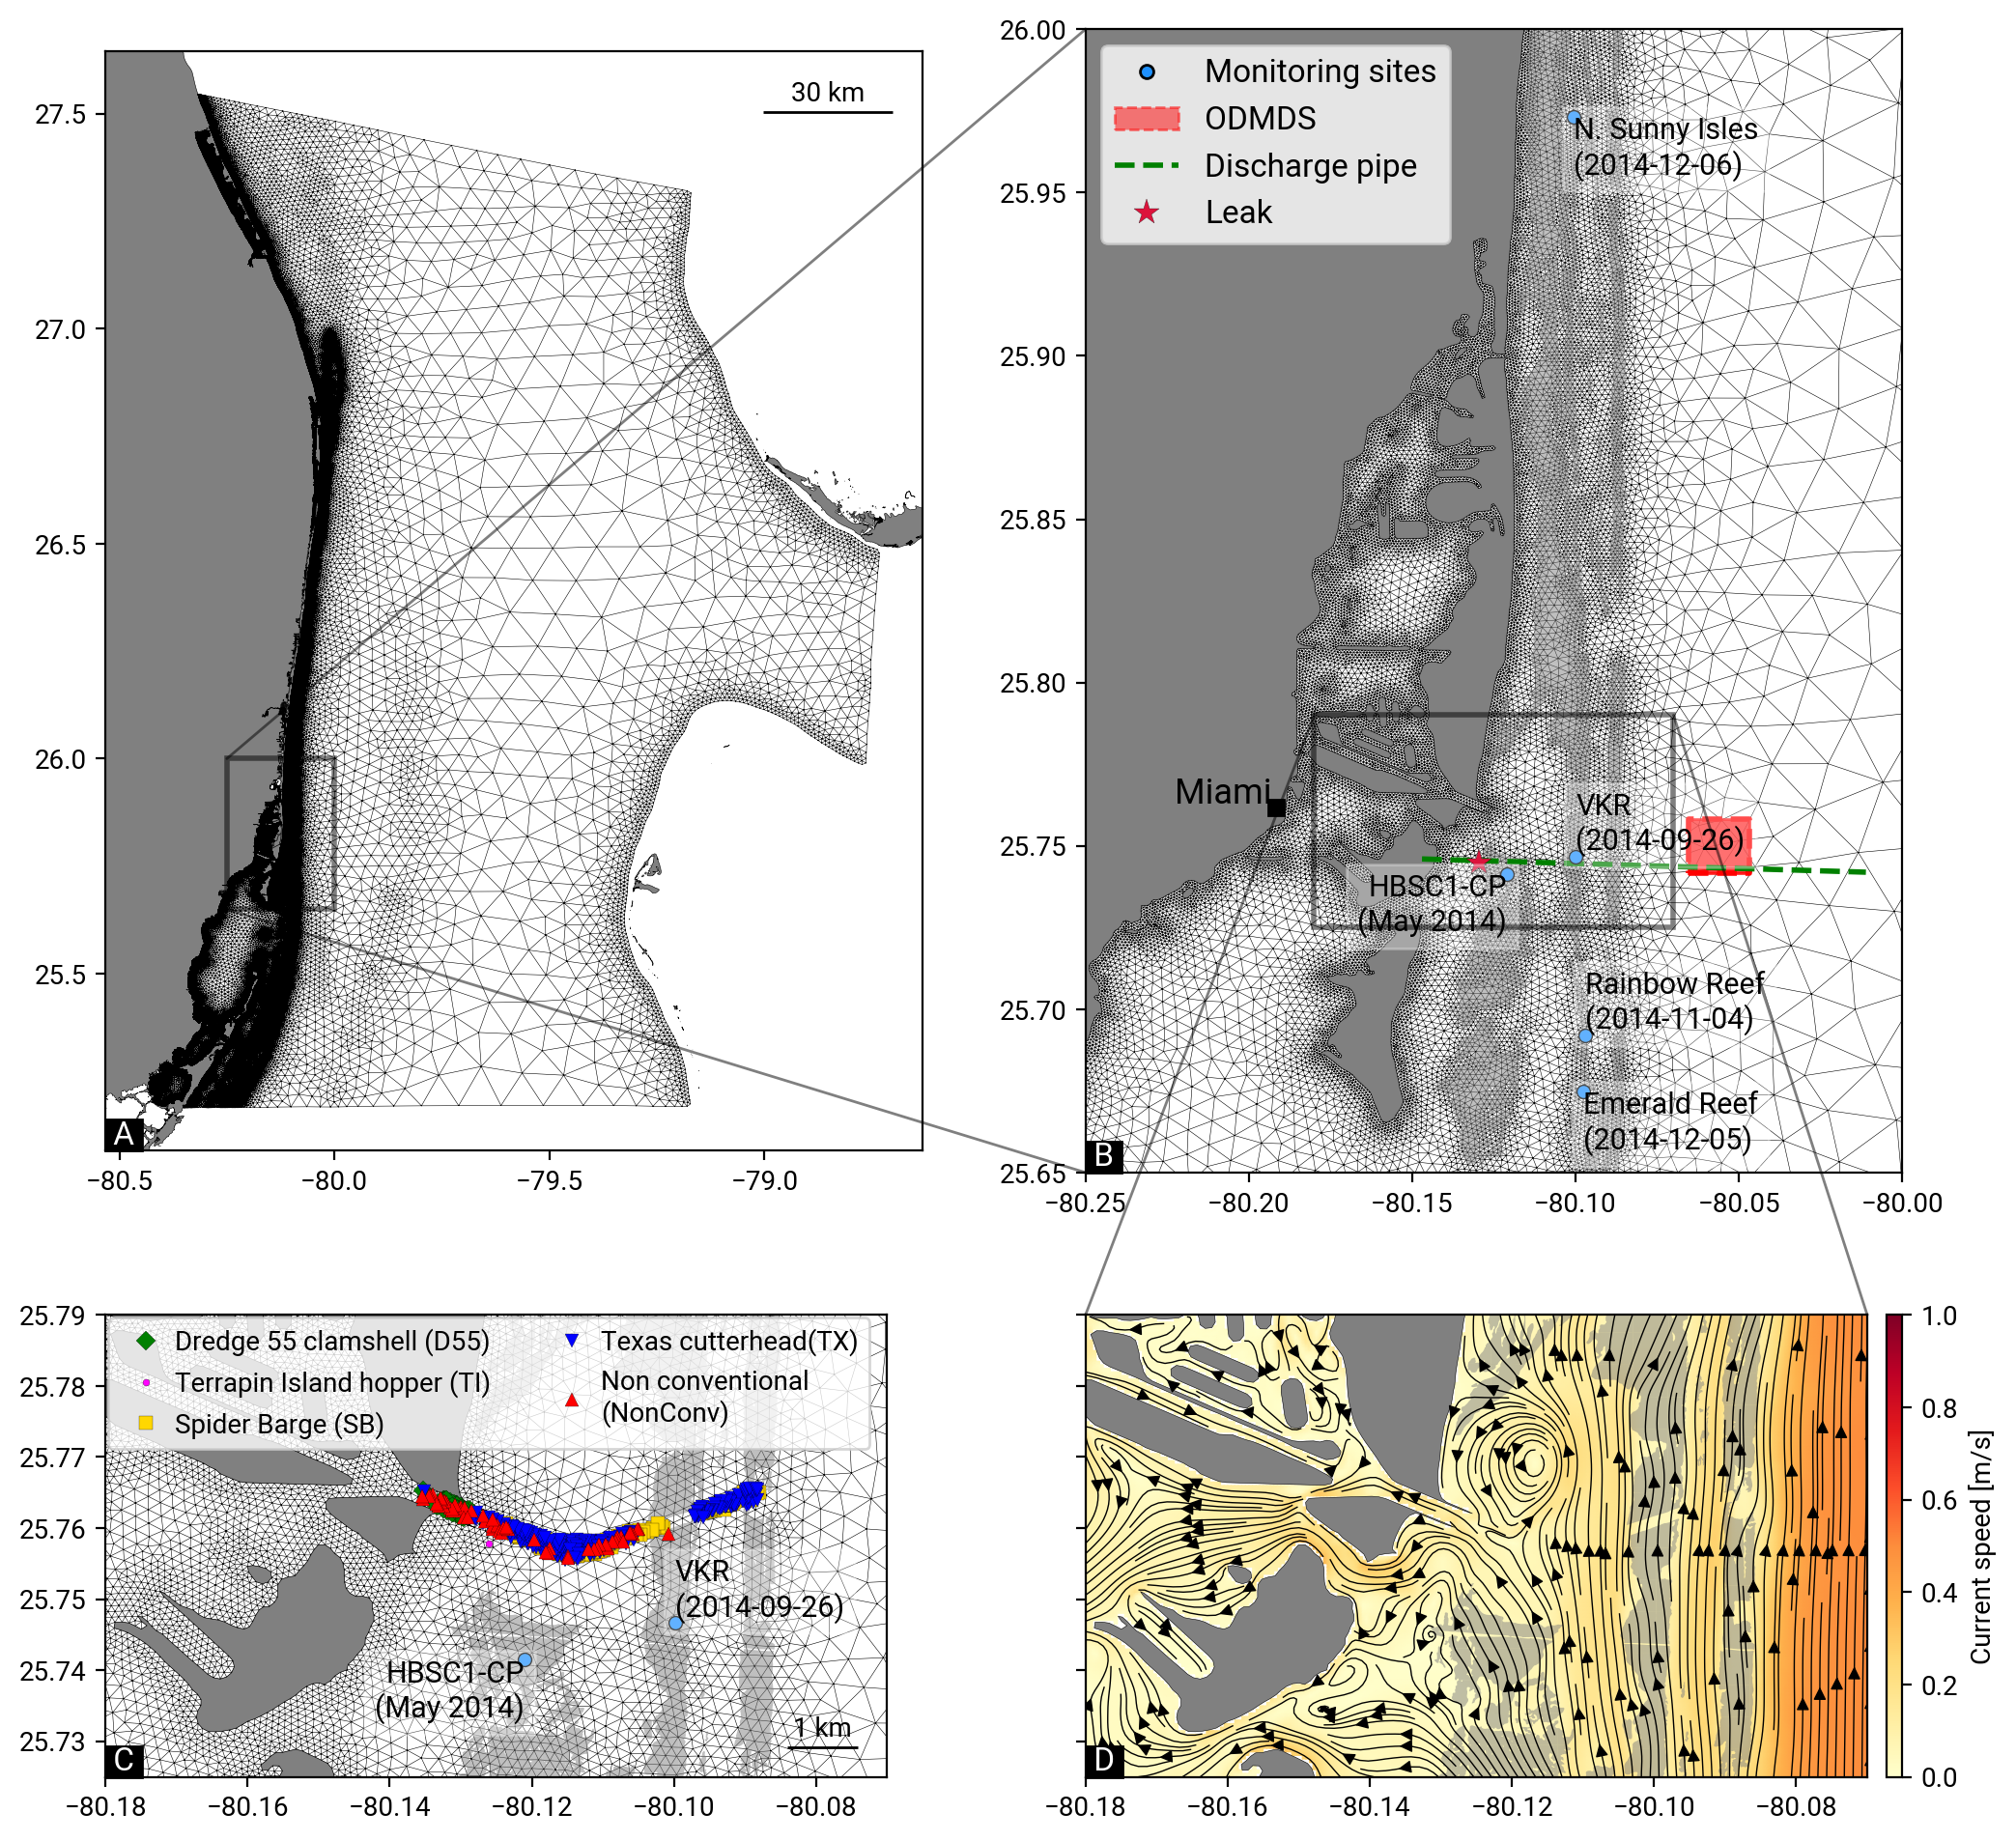
\includegraphics[width=\textwidth]{figures/fig_mesh_new.png}
	\caption{(\textbf{A}) Model mesh near the dredged channel. \modif{The mesh resolution reaches about} 100 m over the reefs (in light grey) and along the coasts (in dark gray). The monitoring sites considered in the present study are shown by light blue dots. The date of the first reported signs of SCTLD at these sites is given between brackets. The Ocean Dredge Material Disposal Site (ODMDS) is shown in red and the discharge pipe of the Miami Central District Municipal Wastewater Treatment Plant in green. (\textbf{B}) Close-up view of the dredged channel. The locations of the different types of dredging that took place during the PortMiami expansion are shown by colored markers. (\textbf{C}) Snapshot of the modeled currents in the vicinity of the dredged channel. Small-scale flow features such as the acceleration of currents between reefs and islands are well reproduced by the model.}
	\label{fig:onset_mesh}
\end{figure}

The hydrodynamics of the entire FCR was modeled using the multiscale ocean model SLIM\footnote{\url{ https://www.slim-ocean.be}}, which has already been extensively validated in the area \citep{frys2020fine,dobbelaere2020coupled,dobbelaere2022impacts,dobbelaere2022connecting}. SLIM uses an unstructured mesh whose resolution can be locally increased in order to accurately represent fine-scale flow features. The mesh used in this study was built following the same methodology as~\cite{dobbelaere2020coupled}, with a local refinement near PoM to achieve a resolution of 100 m in the vicinity of the dredged channel (Fig.~\ref{fig:onset_mesh}A). The mesh consisted of approximately $3.5\times 10^5$ triangles and was generated with the seamsh\footnote{\url{https://pypi.org/project/seamsh/}} Python library, which is based on the open-source mesh generator GMSH \citep{geuzaine2009gmsh}. The model was run between October 15, 2013, and September 26, 2014, with a time step of 10 minutes to cover the whole dredging period prior to the observation of SCTLD at VKR by~\cite{precht2016unprecedented}. The modeled sea surface elevation and currents were exported every hour. Using such a fine mesh resolution, we simulated fine-scale details of the ocean currents, such as the flow acceleration between reefs and islands (Fig. \ref{fig:onset_mesh}C). Atmospheric forcings were obtained from the European Centre for Medium-range Weather Forecasts (ECMWF) ERA-5 dataset and currents were relaxed towards the operational Navy HYbrid Coordinate Ocean Model (HYCOM; \citealp{chassignet2007hycom}) following the approach of~\cite{dobbelaere2022impacts}. The modeled sea surface elevation was validated against tide gauge measurements from station 8723214, located on Virginia Key (see~\ref{onset:validation}).

The transport of sediments released from dredging operations along the channel was then modeled using a Lagrangian transport model, forced by the simulated currents. The sediment transport model is inspired by the Particle Transport Model (PTM), developed by the US Army Corps of Engineers \citep{macdonald2006ptm}. In this model, particles undergo a combination of horizontal and vertical motions. The vertical dynamics is mostly driven by gravity, with heavier particles sinking faster. Once they have settled, particles can be resuspended when shear stress exceeds   the critical Schields parameter, as parameterized by \cite{soulsby1997threshold}. The horizontal motion of the suspended particles is derived from the 2D model velocity by assuming a vertical log profile, hence yielding a quasi-3D approach. Furthermore, to account for the impact wave-induced sediment motion, these current velocity were combined with surface Stokes drift velocity with Breivik's vertical profile \citep{breivik2016stokes}. Stokes drift's velocities were downloaded from Copernicus Marine Services's (CMEMS) Ocean Wave Reanalysis dataset \citep{cmems}. When sediment particles enter the near-bed zone, their horizontal velocity is greatly reduced and sediments are transported with the bed load.

As sediment dispersion is dependent on the grain size, we modeled the dispersal of five sediment classes to represent impacts of fine- to coarse-grained particles: (\textit{i}) 5-50 $\mu$m, (\textit{ii}) 50-100 $\mu$m, (\textit{iii}) 100-200 $\mu$m, (\textit{iv}) 200-300 $\mu$m, and (\textit{v}) 300-400 $\mu$m. We performed a  different simulation for each class, with the grain size randomly drawn from a uniform distribution over the corresponding size range. The density of each sediment particle was derived from its size using the formula of \cite{hamilton1982sound}. Furthermore, all particles were differentiated based on the type of dredge that produced them. Five types of dredge were considered in our modeling study (Fig. \ref{fig:onset_mesh}B): (\textit{a}) Texas cutterhead (TX), (\textit{b}) non-conventional dredging, \ie~TX with suction mechanism turned off (NonConv), (\textit{c}) Spider Barge (SB), (\textit{d}) Terrapin Island hopper (TI), and (\textit{e}) Dredge 55 clamshell (D55).

Dredging operations performed during the expansion of PoM were characterized in our dataset by a date, a location and  a type of dredge (Fig. \ref{fig:onset_mesh}B). In the absence of information about the exact \modif{timing} of the dredging, sediment particles were released from the dredging location during a whole day at a rate of 80 particles/hour in the model. To account for the motion of spider barges between the dredging and disposal sites, particles were released every 500 m along a straight line joining the dredging location to the ODMDS (see Fig. \ref{fig:onset_mesh}A) for every dredging operation labelled as SB.

The potential impact of the modeled sediments on reefs was first evaluated by quantifying the turbidity and sedimentation generated by the different dredging operations over coral reefs. The occurrence of high turbidity over reefs was assessed based on the concentration of suspended sediment particles in the model. This concentration was computed by counting the number of suspended particles inside the cells of a regular 200 m $\times$ 200 m grid over the entire computational domain. The modeled plumes were then compared against daily plume observations derived from satellite imagery by~\cite{cunning2019extensive}\footnote{Datasets available at \url{https://github.com/jrcunning/pom-dredge/}} following the methods of \cite{barnes2015sediment} at sites located within 15 km of the dredged channel. As in these two previous studies, we computed  the simulated plume frequency by dividing the number of days during which plumes occurred by the total number of simulated days for all grid cells. The impact of sedimentation was quantified by computing the cumulated concentration of settled particles within the same computational grid. This cumulated concentration was normalized by the total numbers of simulated time steps and released particles. This normalized concentration gives the averaged fraction of the total mass of particles depositing in each grid cell by unit of area during the simulation. Higher values of this indicator would indicate larger sediment deposition over a longer cumulated time.

The potential impact of dredging on the onset of the SCTLD outbreak was summarized at five monitoring sites where signs of disease were reported. Four sites were reefs where disease was reported in 2014 by~\cite{precht2016unprecedented}. The fifth site was station HBSC1-CP, monitored throughout the expansion of PoM, where \modif{disease signs} were reported in May 2014 (\citealp{dial2017}; Fig. \ref{fig:onset_mesh}A, see~\ref{onset:appendice}) \modif{although it is not clear that this disease was} SCTLD. The impact of dredging was assessed by identifying the dredging operations that produced sediment transported within 500 m of all five sites. We then computed the fraction of the sediment particles produced by these dredging operations that were actually transported within 500~m of the monitoring sites. The 500~m radius was chosen to match the scale of the 500~m $\times$ 500~m reef polygons used in the model \citep{dobbelaere2020coupled}, as well as the mesh size over reefs. The resulting numbers of particles were then divided by the total number of sediment particles released by each type of dredging operation. Larger values of this indicator would suggest a greater impact of a given type of dredging operation at a given monitoring sites.

Additionally, the dispersal of particles was simulated backward in time from VKR and HBSC1-CP to identify the potential sources of pollution affecting these two sites. Ten particles were released from each site every 450 seconds between September 26, 2014, and October 15, 2013, for a total of 673770 particles per site. These simulations aimed at assessing the possibility of pollution by wastewater leaking from the Miami Central District Municipal WWTP discharge pipe \citep{gintert2019regional}. As leaking wastewater particles were expected to be positively buoyant (Precht, \textit{pers. comm.}), there were advected backward in time by a combination of \modif{ocean} currents and surface Stokes drift from CMEMS' Ocean Wave Reanalysis dataset. We then computed risk maps by counting the number of particle trajectories intersecting each cell of a 200 m $\times$ 200 m grid, following the same approach as~\cite{anselain2023qatar}. This number was normalized by the total number of released particles to obtain the probability for each grid cell to be a source of pollution that would reach the monitoring sites.
% Neutral buoyancy of wastewater loads was assumed as a limiting scenario for purposes of this study: observations \citep{bloetscher2014use,wanninkhof2005farfield} suggest that buoyant plumes may transport wastewater several kilometers under prevailing currents and winds in this region.
This probability was then integrated along the wastewater discharge pipe, modeled as a straight line between Miami Central District Municipal WWTP, located on Virginia Key, and the ocean discharge outfall located at 25$^\circ$44'31''N 80$^\circ$05'10''W \citep{koopman2006ocean}.

Finally, as previous studies showed evidence of waterborne transmission of SCTLD \citep{aeby2019pathogenesis, dobbelaere2020coupled,eaton2021measuring, meiling2021variable}, there is a possibility that the disease propagated to VKR from other reefs affected by sediment particles released by non-conventional dredging prior to September 2014. To evaluate this possibility, we computed monthly disease connectivity matrices following the methodology of \cite{dobbelaere2020coupled} during our simulated period. These connectivity matrices can be interpreted as large graphs whose vertices are 500 m $\times$ 500 m sub-reef polygons and whose edges represent disease connectivity pathways. Evaluating the possibility of disease propagation from sub-reefs affected by non-conventional dredging to VKR is therefore equivalent to evaluating the existence of pathways, \ie~sequences of connected vertices in the network starting from these sub-reefs and reaching VKR. As computing all possible pathways is not computationally tractable, we limited ourselves to the computation of shortest paths from the affected reefs to VKR. This was performed using the function \texttt{get\_all\_shortest\_paths} of the Python \texttt{python-igraph} package \citep{csardi2006igraph}. Such a function requires the definition of a weight $w_{ij}$ for the edge connecting reef $i$ to reef $j$. We chose $w_{ij} = 1-\tilde{C}_{ij}$, where $\tilde{C}_{ij}$ is the probability of disease propagation from reef $i$ to reef $j$ computed following the approach of \cite{dobbelaere2020coupled}, so that `shorter' edges of the networks (\ie~connectivity pathways with smaller weights) correspond to connections with a larger disease propagation probability. The probability of a given path was then defined as the mean connection probability of the edges composing this path.


%%%%%%%%%%%%%%%%%%%
% --- RESULTS --- %
%%%%%%%%%%%%%%%%%%%
\section{Results}

% FIGURE 2 - PLUMES
% Plume frequency
% HSBC1-CP:4.14
% VKR: 0.32
% N. Sunny Isles: 19.43
Only grain sizes in the 5-50 $\mu$m range produced plumes consistent with the observations of~\cite{barnes2015sediment} and~\cite{cunning2019extensive} (Fig.~\ref{fig:onset_depo}A). For coarser grain sizes, particles settled in the direct vicinity of the channel. The suspended sediments were then only observed offshore, closer to the Florida Current, where the current velocity was sufficiently strong to prevent deposition. This suggests that the observed turbidity was mostly due to fine silts. With grain sizes of 5-50 $\mu$m, the modeled occurrence of plumes  within 15 km of the dredged matched the presence/absence data of~\cite{cunning2019extensive} in 80.5\% of cases and the total area where plumes were observed was about 205 km$^2$, consistent with the $\sim$228 km$^2$ estimated by~\cite{barnes2015sediment}. Modeled plumes mostly occurred north of the dredged channel, as particles were driven northward under the action of shelf currents influenced by winds and the Florida Current. The highest simulated plume frequency was about 60\% and was found within 1.5~km of the dredged channel, within 1.5~km of the coast of Miami Beach. Plume frequencies of 30-40\% were observed within 4~km north of the dredged channel, between the coasts and the inner reef line. Plumes were observed \modif{during $0.32$~\% of simulated days at VKR site, $4.14$ \% at HBSC1-CP and $19.43$ \% at N. Sunny Isle}. Similarly to~\cite{cunning2019extensive}, we found a positive correlation between plume frequency and sediment deposition, with a Pearson correlation coefficient of \modif{0.29}.

% \begin{table}
%     \centering
%     \begin{tabular}{|l|cccc|}
%         \hline
%          & Threshold         & Accuracy & False positive  & False negative \\
%          & [particles/m$^2$] & [\%]     & [\%]            & [\%]  \\
%         \hline
%         5-50 $\mu$m    & 21 & 86.678 & 2.912 & 10.410 \\
%         50-100 $\mu$m  & 20 & 83.058 & 8.525 & 8.417 \\
%         100-200 $\mu$m & 30 & 84.814 & 7.133 & 8.053 \\
%         200-300 $\mu$m & 18 & 84.459 & 7.988 & 7.553 \\
%         300-400 $\mu$m & 13 & 84.615 & 8.140 & 7.244 \\
%         \hline
%     \end{tabular}
%     \caption{Validation of the modeled presence of plumes against plume observations from satellite imagery. Overall, the model agrees well with observations}
%     \label{tab:onset_val}
% \end{table}

\begin{figure}
	\centering
	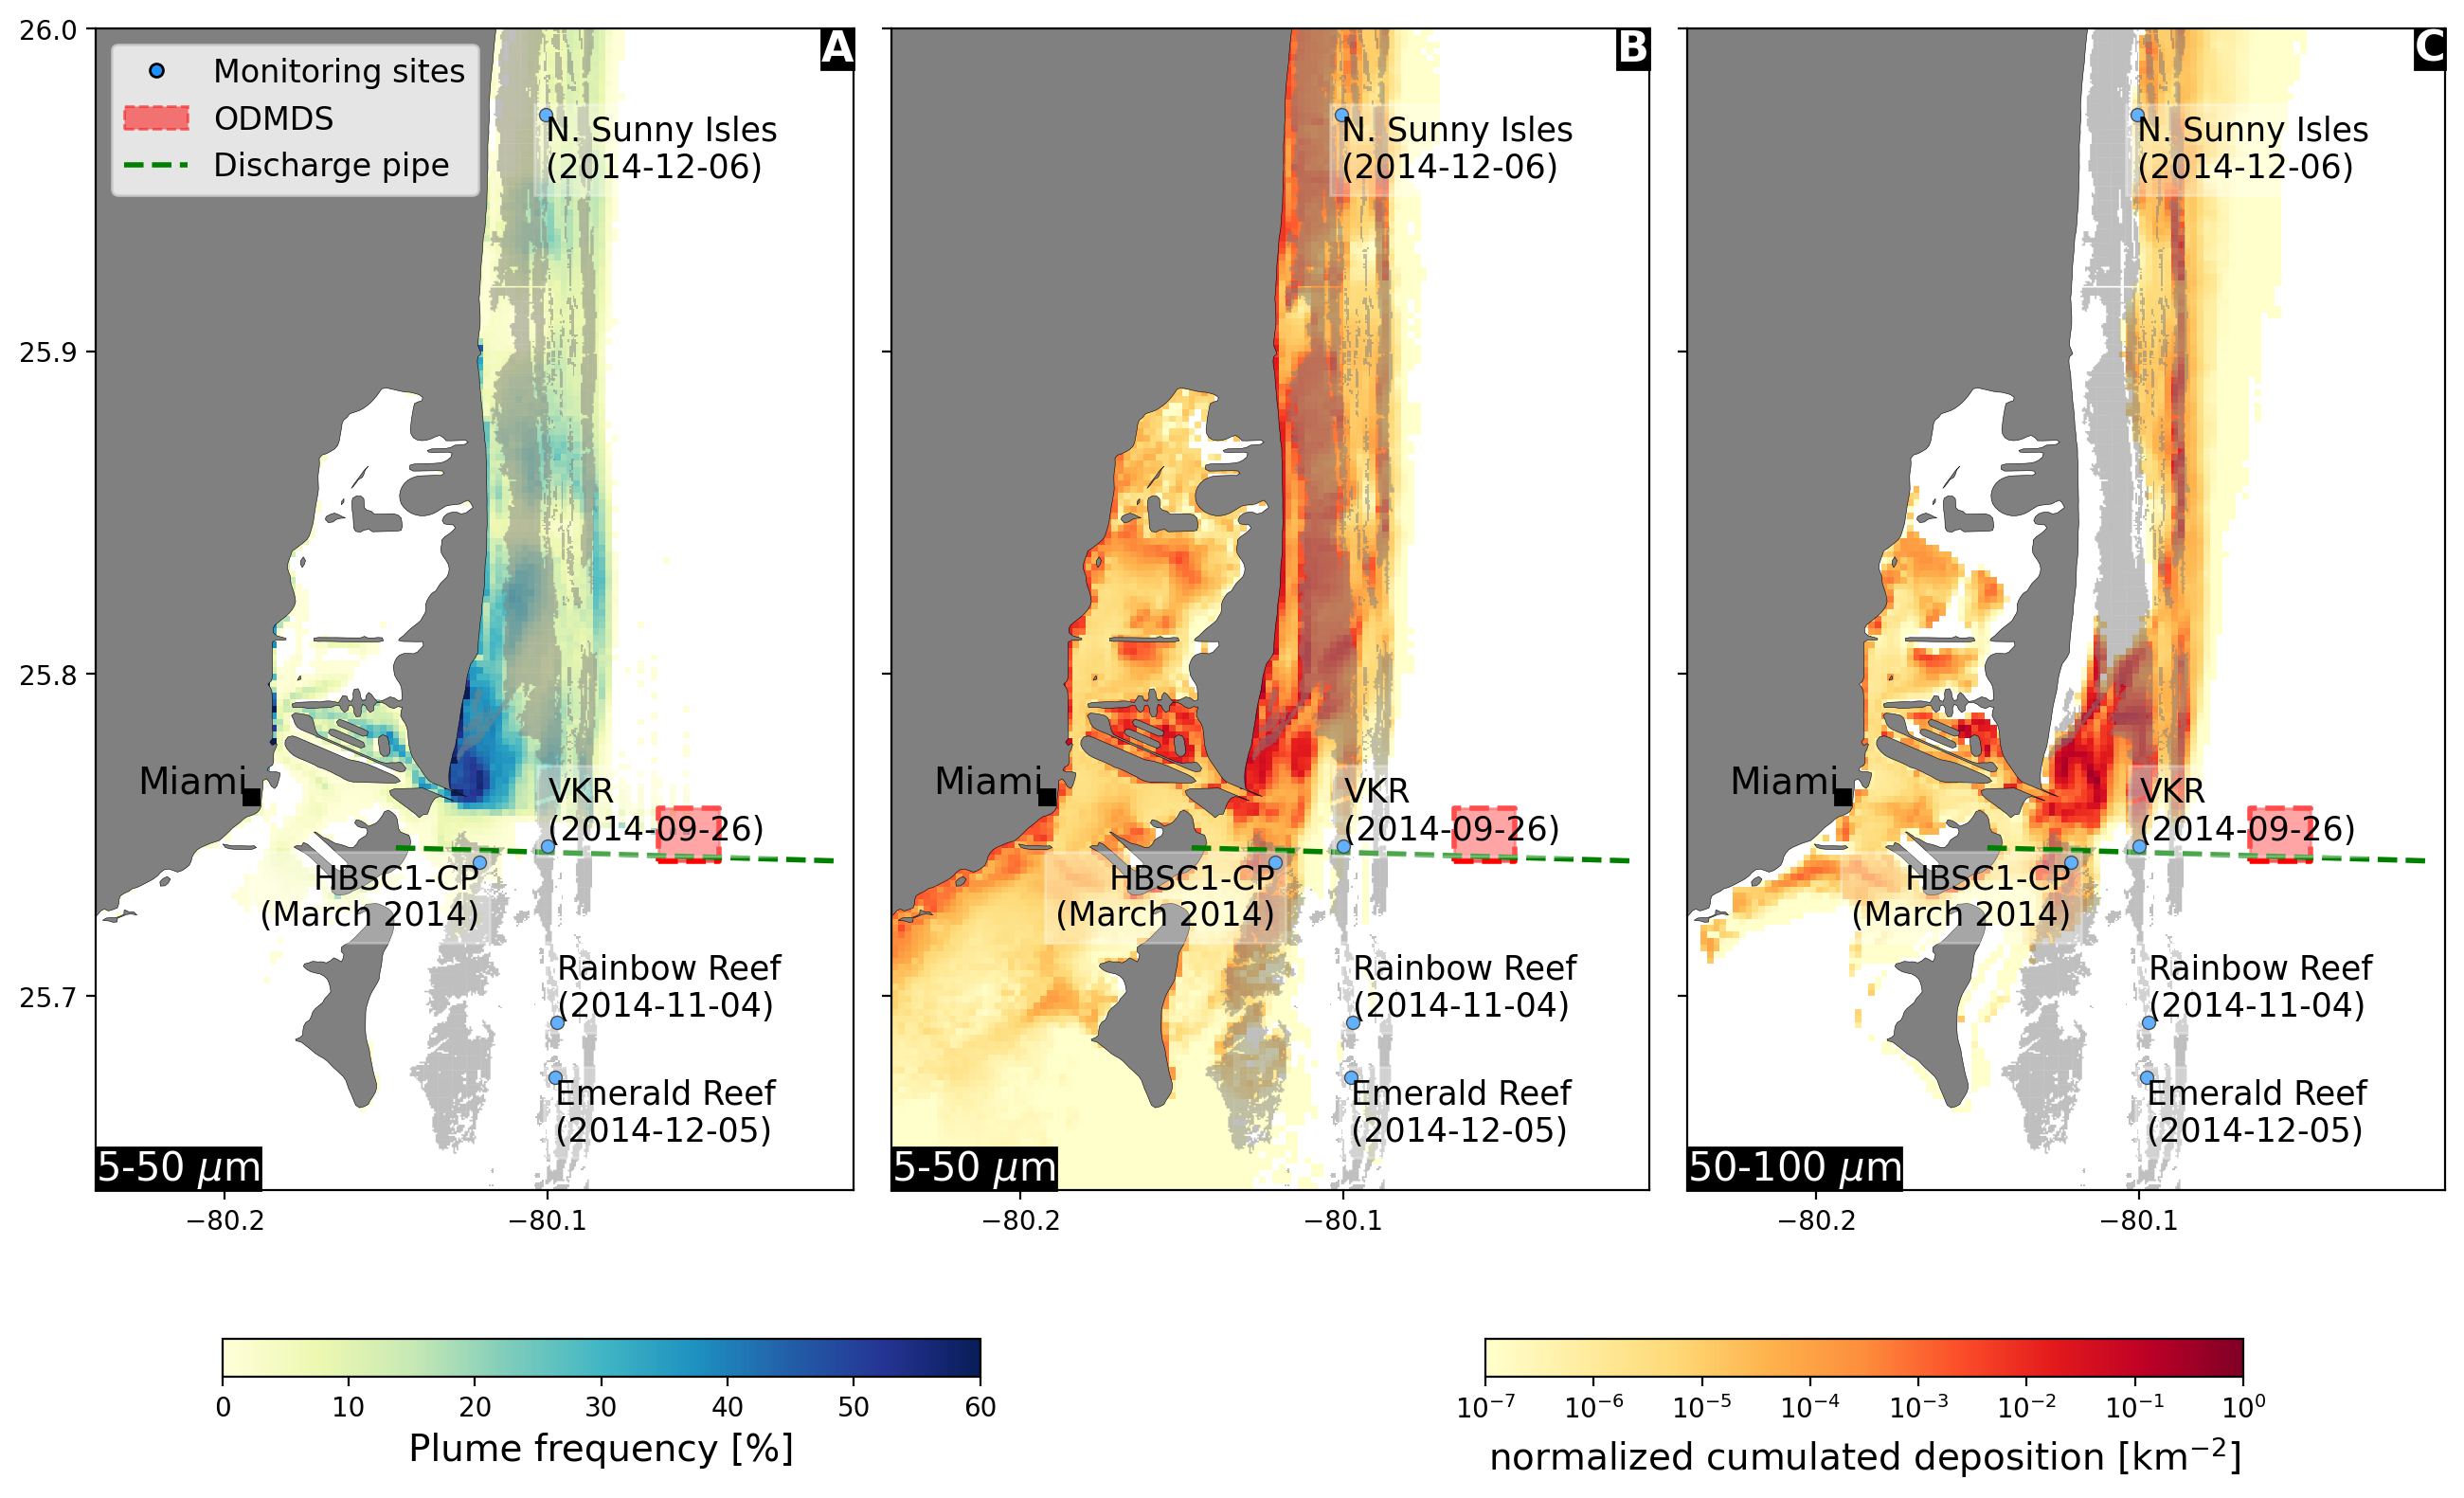
\includegraphics[width=\textwidth]{figures/fig2_stokes4.png}
	\caption{\textbf{(A)}: Plume frequency for grain size in the range 5-50 $\mu$m. The averaged concentration of deposited sediments are shown for grain sizes more likely to carry the disease: \textbf{(B)} 5-50 $\mu$m and \textbf{(C)} 50-100 $\mu$m. Most modeled turbidity and sedimentation occurred north of the dredged channel.}
	\label{fig:onset_depo}
\end{figure}

% FIGURE 2 - DEPOSITION
% Site           | Class 1 |  Class 2
% VKR            | 3.23e-6 | 7.63e-6
% HBSC1-CP       | 8.64e-4 | 1.386e-3
% N. Sunny Isles | 2.25e-4 | 5.72e-4
% Rainbow Reef   | 4.4e-7  | NA
% Emerald Reef   | 4.53e-9 | NA
Deposition results are shown for grain sizes corresponding to silts, which are more likely to carry organic matter and therefore more likely to carry SCTLD agents \citep{erftemeijer2012environmental}(Fig.~\ref{fig:onset_depo}B,C). Sedimentation mostly occurred on reefs located north of the dredge channel, although some sediment particles deposited along the coastlines of Virginia Key, Key Biscayne and Miami for all modeled grain sizes. For grain sizes finer than 50~$\mu$m, sediments mostly settled on inshore reefs and along coastlines, while sedimentation mostly took place on offshore reefs for grain size coarser than 50~$\mu$m. Furthermore, sediment particles finer than 50 $\mu$m, deposited further south and west, with deposition occurring over all the area between mainland Florida and the reef line. On average, the fraction of all sediments released depositing at \modif{ VKR, HBSC1-CP and N. Sunny Isles was respectively $3.23\times10^{-6}$ km$^{-2}$, $8.64\times10^{-4}$ km$^{-2}$ and $2.25\times10^{-4}$ km$^{-2}$ for grain sizes of 5-50 $\mu$m, and $7.63\times10^{-6}$ km$^{-2}$, $1.39\times10^{-3}$ km$^{-2}$ and $5.72\times 10^{-4}$ km$^{-2}$} for grain sizes of 50-100 $\mu$m. The deposition at these two sites therefore decreased with increasing grain sizes. \modif{Additionally, the fraction of the total particle mass depositing at Rainbow Reef and Emerald Reef was respectively $4.4\times10^{-7}$ km$^{-2}$ and $4.53\times10^{-9}$ km$^{-2}$ for grain sizes of 5-50 $\mu$m, while no sedimentation occurred at these sites for grain sizes of 50-100 $\mu$m.}

% FIGURE 3
The sediment particles with grain size 5-50~$\mu$m (resp. 50-100~$\mu$m) released by $99$ \% (resp. $83$~\%) of all simulated dredging operations reached N Sunny Isles, making it the reef site most impacted by the simulated dredging operations (Fig.~\ref{fig:onset_bar}). HBSC1-CP was the second most impacted site and was affected by $43$~\% (resp. $35$~\%) of dredging operations with grain sizes of 5-50~$\mu$m (resp. 50-100~$\mu$m). VKR \modif{was the third most impacted site and received sediments from $12.4$~\% (resp. $4.6$~\%) of dredging operations with grain sizes of 5-50~$\mu$m (resp. 50-100~$\mu$m). Finally, Rainbow Reef and Emerald Reef were impacted by $<4.5$~\%~\% (resp. $<0.5$~\%) of dredging operations with grain sizes of 5-50~$\mu$m (resp. 50-100~$\mu$m)}. Most modeled sediment particles ($>90$~\%) were not transported within 500~m of the reef sites, and the fraction of particles reaching the monitoring sites decreased with increasing grain sizes. \modif{Nonetheless, N. Sunny Isles, VKR and HBSC1-CP were all impacted by non-conventional dredging for the two considered grain size classes. When considering the non-conventional dredging operations, VKR, HBSC1-CP and N. Sunny Isles were respectively affected by $1.17$~\%, $4.37$~\% and $14.80$~\% of the released sediments for grain sizes of 5-50~$\mu$m, and $0.38$~\%, $2.19$~\% and $3.36$~\% for grain sizes of 50-100~$\mu$m.} However, as non-conventional dredging was expected to release more sediments in the water column than conventional dredging operations where dredged material was collected, this relative metrics might underestimate the impact of non-conventional dredging operations.

\begin{figure}
	\centering
	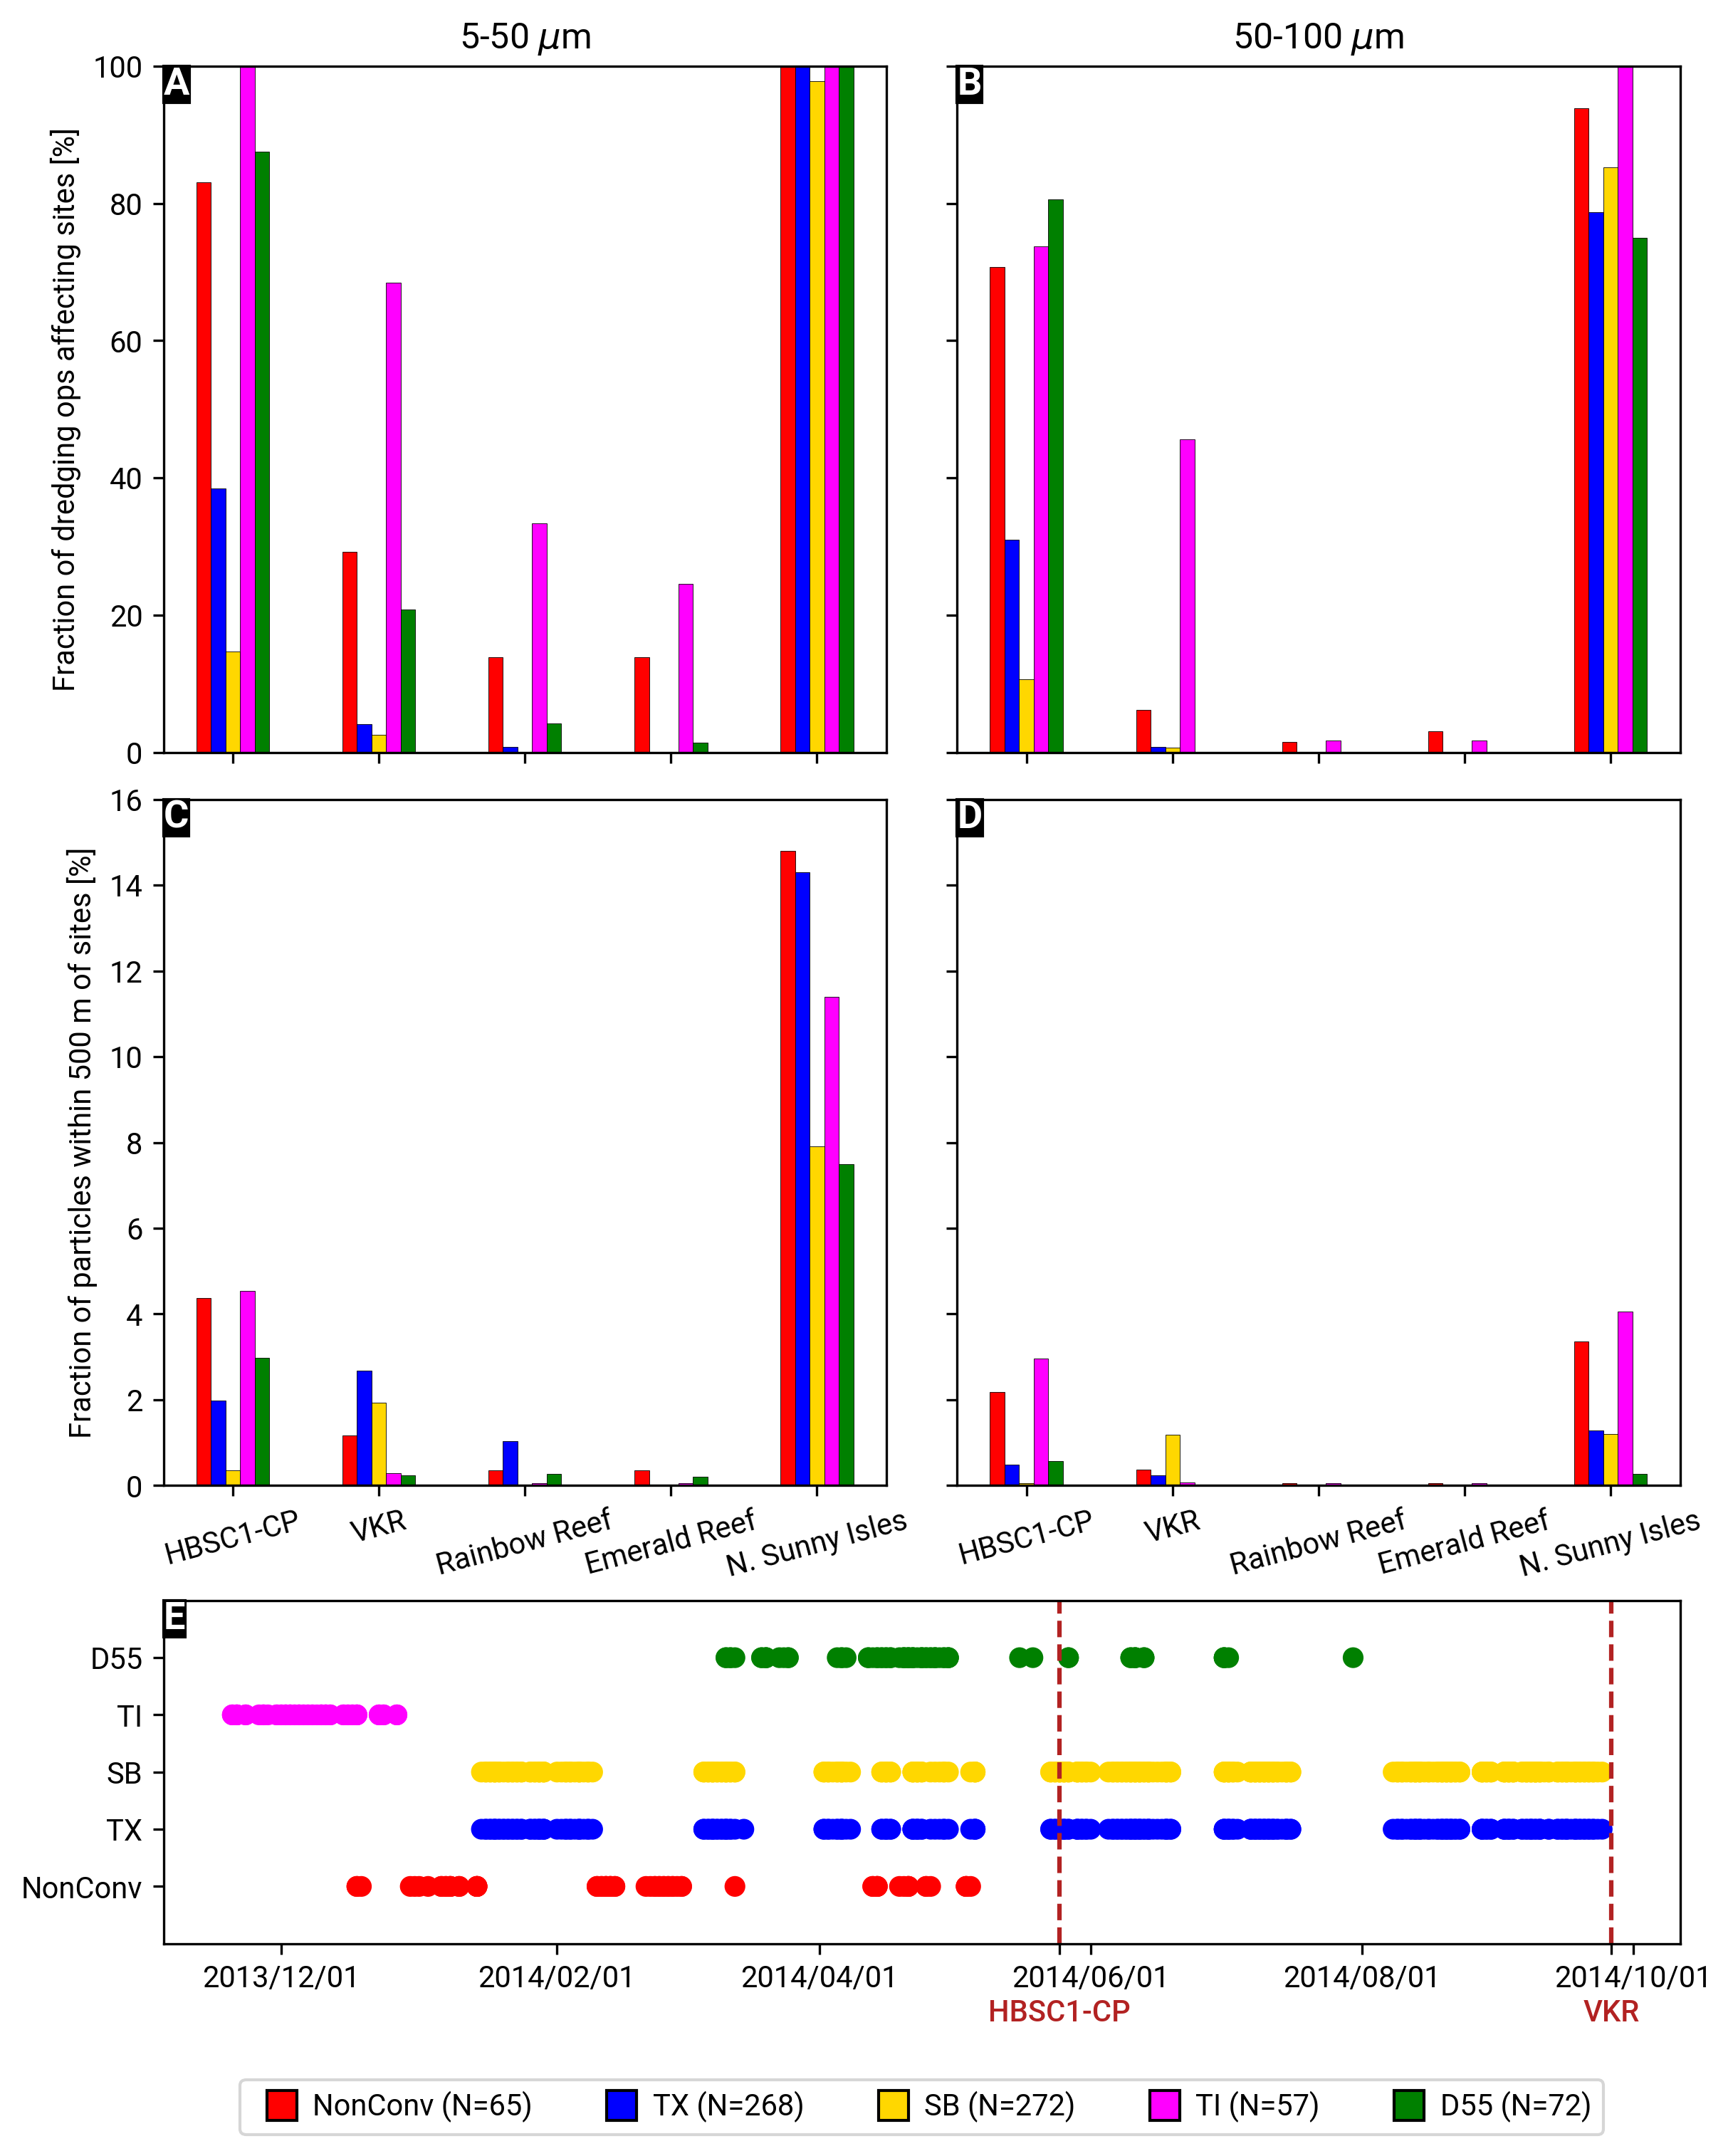
\includegraphics[width=.85\textwidth]{figures/aggregated_stokes4_v3_500m_timeline_rel.png}
	\caption{Fraction of simulated dredging operations producing sediment particles that were transported within 500~m of HBSC1-CP, VKR and N. Sunny Isles for grain sizes of (\textbf{A}) 5-50 $\mu$m  and (\textbf{B}) 50-100 $\mu$m. Fraction of the sediment particles produced by these operations transported within 500~m of HBSC1-CP, VKR and N. Sunny Isles for grain sizes of (\textbf{C}) 5-50 $\mu$m  and (\textbf{D}) 50-100 $\mu$m. \textbf{E}: Temporal distribution of the simulated dredging operations. The dates of the first reported disease signs at HBSC1-CP and VKR site are shown with dotted dark red vertical lines. The total number of simulated dredging operations (N) is given between brackets for each dredging type. N. Sunny Isles was the most affected site. All sites were impacted by non-conventional dredging for the two considered grain sizes}\label{fig:onset_bar}
\end{figure}

% FIGURE 4
When considering wastewater pollution, backtracking of particles from HBSC1-CP and VKR suggest that the most probable source of pollution to these sites were located within narrow `cones' directly south of their location (Fig.~\ref{fig:backtrack}). Inside these cones, the probability for pollutants to reach the sites decreases southward with the distance to the sites and drops below 30\% 300~m away, below 10\% after 1-1.5~km, below 5\% after 3~km, and below 1\%  15~km away from the sites. Outside of these cones, the probability to reach VKR and HBSC1-CP quickly decreases below 1\%. This suggests that it was possible (although with a low probability) for positively buoyant non-sediment pollutants coming from Miami or the dredged channel to reach the monitoring sites. Integrating the probability of arrival along the wastewater discharge pipe, we find that the probability for pollutants leaking from the pipe to reach HBSC1-CP (located south of the pipe) was below 5\% within 2~km of the site and then dropped below 1\%. However, the probability for leaking pollutants to reach VKR site (located north of the pipe) was up to 40\% at the position of the site and dropped below 1\% 500~m away from the sites. This suggests that pollutant leaking from the pipe was unlikely to affect HBSC1-CP and unlikely to affect VKR unless the leak was located within $500$~m of VKR.

\begin{figure}
    \centering
    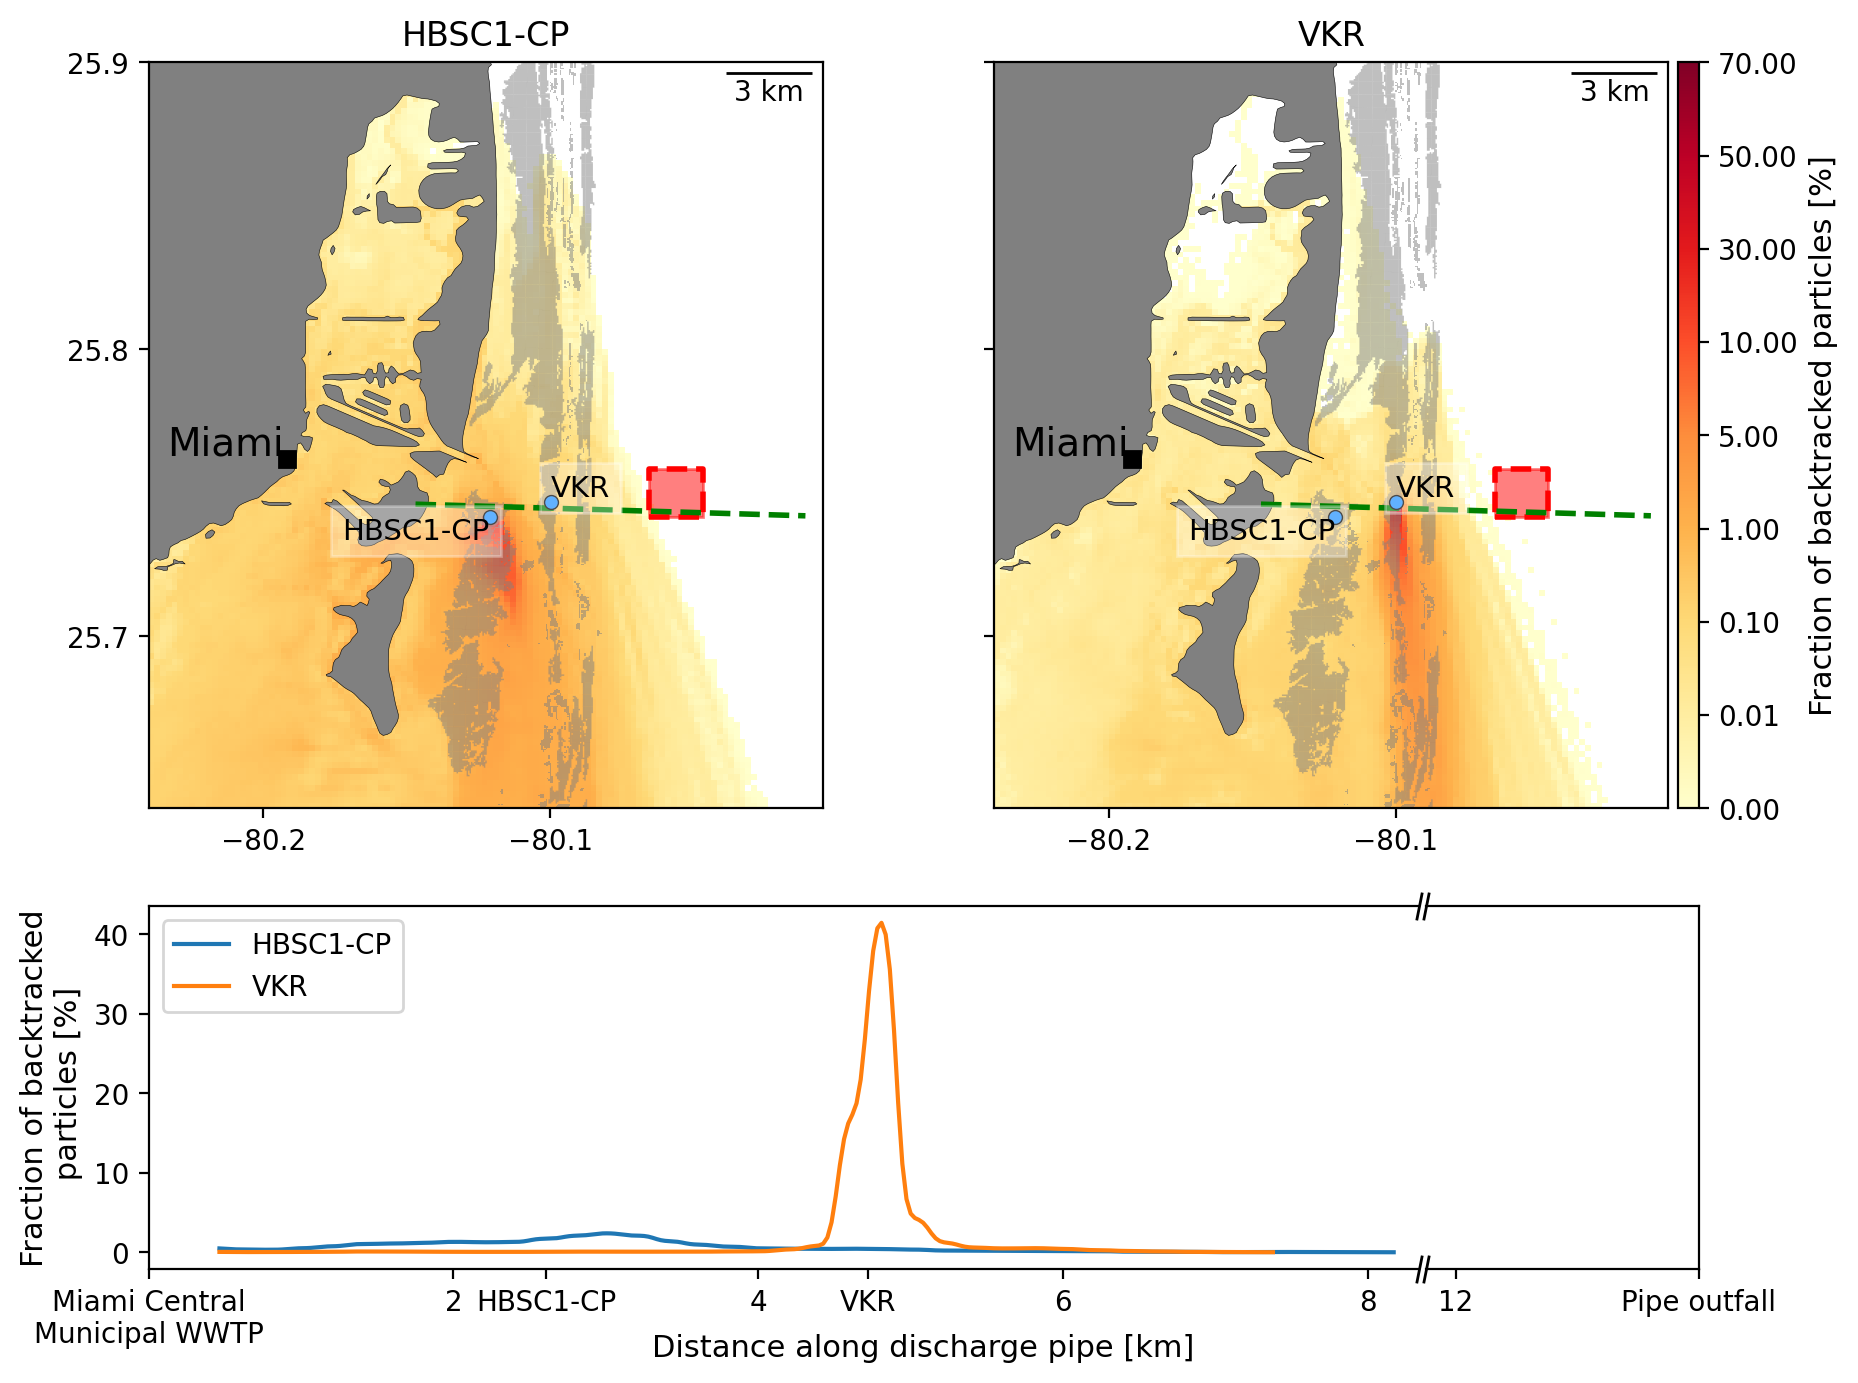
\includegraphics[width=.98\textwidth]{figures/fig_proba_stokes_v2.png}
    \caption{Spatial distribution of the probability to be a source of positively buoyant pollutants reaching HBSC1-CP (\textbf{top left}) and VKR (\textbf{top right}). \textbf{Bottom}: Integration of this probability along the discharge pipe of Miami Central District Municipal WWTP, which was reported to leak in 2017. Most likely sources of pollutants were located within a few kilometers south of HBSC1-CP and VKR.}
    \label{fig:backtrack}
\end{figure}

% FIGURE 5
\modif{We assessed the presence of shortest paths from reefs affected by non-conventional dredging to VKR in the modeled monthly disease connectivity networks between May and September 2014 (Fig.~\ref{fig:onset_path})}. \modif{These affected reefs include HBSC1-CP, where potential disease signs were reported in May 2014}. We found connectivity pathways \modif{to VKR} during all months of May-September 2014. This suggests that there was a possibility of disease propagation \modif{from the reefs affected by non-conventional dredging operations} to VKR during all of these 5 months. However, we found no direct pathway \modif{connecting HBSC1-CP to VKR}. Southern intermediary reefs were systematically needed as stepping stones for the propagation of the disease. This suggests that several months might have been required for disease agents to reach VKR from HBSC1-CP. \modif{Nonetheless, the structure of the connectivity pathways remained fairly similar during the five simulated months, indicating favorable conditions for disease propagation to VKR over several months.}
% * <thomas.dobbelaere@uclouvain.be> 13:26:22 18 May 2022 UTC+0200:
% Lew: should be justify why no observation of SCTLD at VKR in the meantime

\begin{figure}
	\centering
	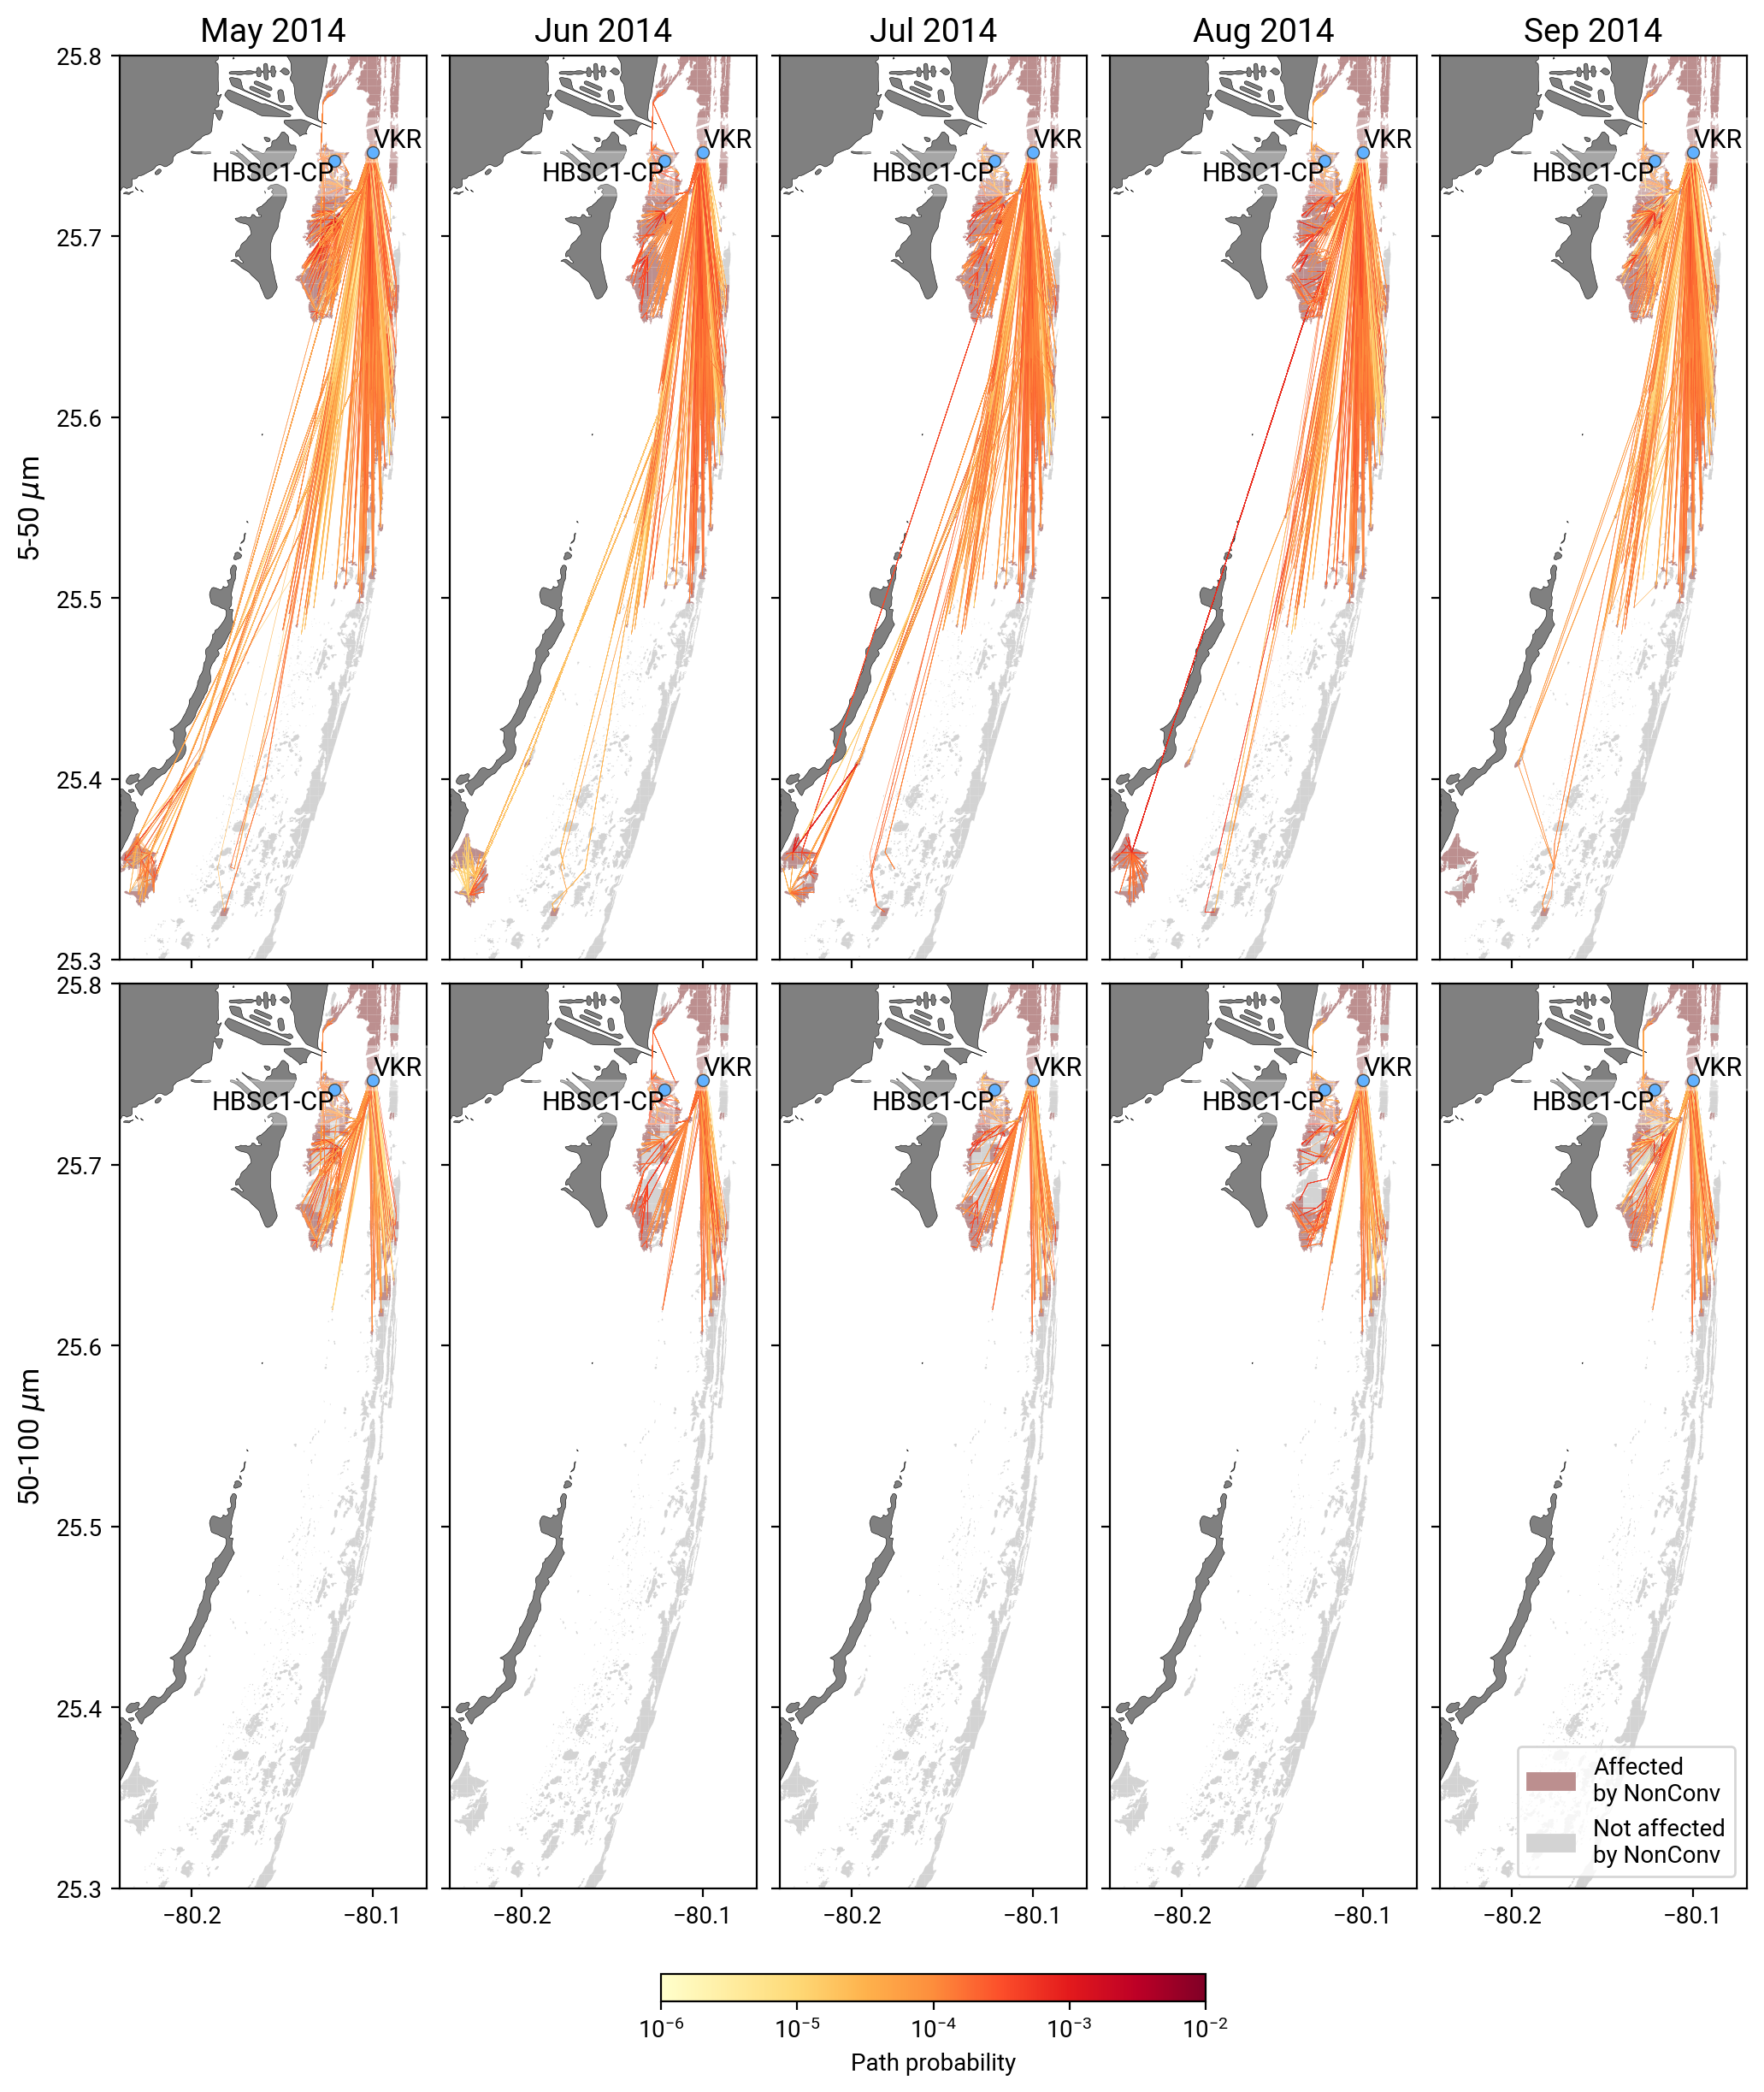
\includegraphics[width=\textwidth]{figures/figure_new_shortest_paths.png}
    \caption{Shortest path from the reefs affected by non-conventional dredging to the monitoring site near Virginia Key (VKR) in the monthly disease connectivity networks between May and September 201. Southern intermediary reefs were needed as stepping stones for the propagation of the disease to VKR.}
	\label{fig:onset_path}
\end{figure}

% === DISCUSSION === %
\section{Discussion}

% Importantly, this study only considered two possibilities that may have contributed to the SCTLD outbreak: dredging activities and a pollutant leak. Among these two options, there is more support for dredging than a pollutant leak because the probabilities that pollutants reached sites where SCTLD was possibly first observed were lower than the probabilities of sediment from dredging reaching the same sites; no leaks were reported in this early period; and the area was monitored well. Additionally, we cannot rule out HSCB1-CP as a potential source for the SCTLD outbreak over VKR because connectivity matrices demonstrate SCTLD could have reached VKR via stepping stones; and HSCB1-CP would have received more sediment from dredging than VKR if dredging is in fact the causative agent.”

% SUMMARY
Using a high-resolution quasi-3D sediment model, we reproduced a sediment dynamics consistent with plume observations derived from satellite imagery and in-water observations of sediment deposition at selected sites. Our results suggest that sediment particles produced by dredging were mostly transported northward under the influence of the Florida Current. \modif{Dredging operations had limited impacts on the southern sites of Rainbow Reef and Emerald Reef, while up to $12$~\% of dredging had a direct impact on VKR, identified as the site where the outbreak of SCTLD was initiated in September 2014 \citep{precht2016unprecedented}}. Furthermore, our results indicate that it is unlikely that VKR was affected by pollutants leaking from the discharge pipe of Miami Central District Municipal WWTP unless the leak was located within 500 m from the sites, while HBSC1-CP was very unlikely to receive pollutants leaking from the pipe. \modif{Signs of disease (that may or may not be SCTLD) were observed prior to September 2014 at HBSC1-CP, where both sediment plumes and deposition occurred in the simulations. Furthermore, monthly disease connectivity networks indicate that disease agents could have been transmitted from reefs affected by non-conventional dredging operations} to the site of VKR through multistep connectivity pathways.

% LARGE IMPACT OF DREDGING
Our study confirms previous reports about the widespread impact of the expansion of PoM. As in \cite{barnes2015sediment}, the total area of plumes in our model was about 205 km$^2$. Furthermore, our model reproduced the plume presence/absence within 15 km of the dredged channel derived by \cite{cunning2019extensive} with an accuracy of 80.5\%. Such a good agreement was only obtained for grain sizes in the range 5-50 $\mu$m, suggesting that fine silts were the main drivers of the turbidity generated by dredging, which is consistent with previous studies \citep{storlazzi2015influence,fourney2017additive}. Despite this good agreement, the distribution of plumes predicted by our model tends to be shifted northward compared to these previous studies. These discrepancies might be explained by the fact that our approaches is solely based on sediment concentration. However, turbidity depends on many local factors such as the water content of phytoplankton and organic matters \citep{gray2000comparability,thackston2000improved}. As reported by \cite{cunning2019extensive}, we found a positive correlation between sedimentation and plume frequency. As areas with higher cumulated sediment deposition were mostly located over coral reefs, our results suggests that the expansion of PoM likely harmed coral populations over an extended area through increased turbidity and sedimentation. This sedimentation mostly took place on nearshore reefs with grain sizes finer than 50 $\mu$m and on offshore reefs with coarser grain sizes. Sediment settlement might be significantly harmful to offshore coral reefs populations as they are usually less accustomed to sedimentation than their inshore  counterparts \citep{wolanski2005fine}.

% LIMITATION ABOUT AMOUNT OF RELEASED SEDIMENTS
A limitation of our study is that conventional and non-conventional dredging operations are treated in the same way in the model. For all dredging types, sediment particles were released at the same rate in the model. Although conventional dredging was reported to release fine-grained sediments in the water column through dewatering and barge overflow \citep{jones2016assessing}, the quantity of dredged material lost in the water was limited by the use of pumping mechanisms. In contrast, for non-conventional dredging, the suction mechanism was turned off, causing all chopped rock particles to be released in the water column. The numbers of particles reaching the monitoring sites were therefore likely underestimated for non-conventional dredging operations. However, the fractions given in Fig. \ref{fig:onset_bar}C,D remain valid as they are relative to the total amount of sediment released in the water column for each type of dredging operation. When considering the finest modeled grain size, VKR, HBSC1-CP and N. Sunny Isles were respectively affected by 29\%, 83\% and 100\% of the non-conventional dredging operations that took place between December 2013 and May 2014. Furthermore, HBSC1-CP exhibited the highest deposition of sediments produced by non-conventional dredging. These sediment particles therefore had a higher probability to settle and to be in direct contact with corals. In addition to smothering corals and diverting their energy through sediment removal \citep{erftemeijer2012environmental}, these settled sediments spend more time in direct contact with the corals and might therefore yield a stronger disease transmission potential.

% The coral reefs of N. Sunny Isles appeared to be highly exposed to fine-grained sediments produced by dredging (Fig. \ref{fig:onset_bar}). Furthermore, the non-conventional rock-chopping that took place between December 2013 and May 2014, was a non-negligible source of sediments to N. Sunny Isles, as up to 17\% of the released particles reached the site. As sediments have the potential to act as a SCTLD vector \citep{rosales2020rhodobacterales, studivan2022reef}, the dredging might therefore have contributed to the observed onset of the disease on the reefs of N. Sunny Isles in June 2014, if these sediments contained disease inducing agents. Moreover, up to 3\% of the fined-grained sediments produced by non-conventional dredging reached the site HBSC1-CP before May 2014, when the disease was first reported there. Although this represents a more limited quantity of sediments, HBSC1 was within 2 km from the sites where non-conventional dredging took place, in a region where the model predicted significant sedimentation. Therefore, although a smaller fraction of sediments reached HBSC1-CP, they had a higher probability to settle and to be in direct contact with corals. In addition to smothering corals and diverting their energy through sediment removal \citep{erftemeijer2012environmental}, these settled sediments spend more time in direct contact with the corals and might therefore yield a stronger disease transmission potential.
% * <thomas.dobbelaere@uclouvain.be> 15:28:44 18 May 2022 UTC+0200:
% Same  comment reg. "reached"

% POSSIBILITY OF DISEASE PROPAGATION THROUGH WATERBORNE TRANSMISSION
\modif{Results from sediment simulations suggest that up to $29$~\% of the simulated non-conventional dredging operations has a direct impact on VKR,} identified as the site where the outbreak was initiated in September 2014 \citep{precht2016unprecedented}. Furthermore, backtracking of positively buoyant pollutants from VKR suggests that the probability of reaching the site quickly decreased below 1~\% for pollutant sources that were not located directly south of VKR. When integrating this probability of arrival along the discharge pipe of Miami Central District Municipal WWTP, we found that contamination by leaking wastewater particles was unlikely unless the leak was located within hundreds of meters of VKR. Additionally, the discharge pipe was only reported to be leaking in 2017 \citep{staletovich2017} and there is therefore no evidence that there was a leak before September 2014. However, signs of disease were observed prior to September 2014 at the sites of HBSC1-CP, which was more strongly impacted by the dredging. Although there is no evidence that these were signs of SCTLD, we did not rule out this possibility and investigated the potential for waterborne disease transmission from HBSC1-CP to VKR. We built and analyzed monthly disease connectivity networks and found connectivity pathways from \modif{reefs affected by non-conventional dredging operations, including HBSC1-CP} to VKR \modif{between May and September} 2014. This implied that the propagation of the disease from \modif{these reefs} to VKR through hydrodynamics-driven transport of disease agents was possible during these \modif{five} months. All pathways \modif{connecting HBSC1-CP to VKR}  used reefs located further south as stepping stones. Therefore, the propagation of SCTLD to VKR starting from HBSC1-CP required these intermediary reefs to be first infected by disease agents released from HBSC1-CP. Once diseased, these colonies would then send disease agents to affect the next colonies of the connectivity pathway until the outbreak reached VKR. Assuming an averaged transmission time of the order of 5-10 days \citep{dobbelaere2020coupled}, disease propagation from HBSC1-CP to VKR might have required several months. This is consistent with the 5-month period separating disease reports at these two sites. Moreover, the fact that connectivity pathways \modif{with similar structures were observed between May and September 2014} suggests that disease propagation could indeed have occurred over several months without being interrupted by changing hydrodynamic conditions.
% * <thomas.dobbelaere@uclouvain.be> 15:40:18 18 May 2022 UTC+0200:
% Idea ? Link statement about impact of sediments at VKR with Gintert et al. (2019) ?

\section{Conclusion}

In the present study, we considered different scenarios of disease transmission to the reef sites where SCTLD was first reported, considering uncertainties about the timing and occurrence of the disease at two of these sites. We first evaluated the impact of the dredging operations that took place during the deepening of the Port of Miami shipping channel on the neighboring coral reefs. This was performed using a quasi-3D sediment model forced by high-resolution currents from the multiscale coastal ocean model SLIM. As the first reported signs of SCTLD were coincident with the PMDDP and since sediments may be a SCTLD vector, we wanted to evaluate the fraction of sediments produced by the PMDDP that reached VKR and other monitoring sites where the disease was reported. Second, as two of the considered reef sites were located in the direct vicinity of the discharge pipe of the Miami Central District Municipal Wastewater Treatment Plant, we assessed the vulnerability of these sites to pollutants leaking from the pipe. Finally, we evaluated the possibility of waterborne transmission of SCTLD to VKR from other reefs impacted by the dredging, assuming that these reefs were indeed affected by SCTLD. When modeling the potential sediment transport, we paid special attention to the sediments produced by non-conventional rock chopping during which pumping mechanisms were turned off, causing all chopped rock particles to be directly released in the water column.

Our results suggest that the dredging operations, including non-conventional dredging, had non negligible direct impact on VKR. This indicates that direct disease transmission by sediments to VKR was possible. Furthermore, our results show that these dredging operations also had a non-negligible impact on the sites of N. Sunny Isles and HBSC1-CP, where signs of a disease that could be SCTLD might have been observed before the outbreak was first reported at site VKR. This suggests that the sediments might also have triggered the onset of the disease at these two sites. However, the results of our transport model indicate that leaking pollutants were not likely to affect the reef sites located near the wastewater discharge pipe. Furthermore, using a previously developed bio-physical model that successfully reproduced the observed spread of SCTLD, we show that, assuming that the disease observed at site HBSC1-CP was SCTLD, there was a possibility of waterborne disease propagation from HBSC1-CP to the reefs of Virginia Key.

Importantly, this study only considered two possibilities that may have contributed to the SCTLD outbreak: dredging activities and a pollutant leak. Among these two options, there is more support for dredging than a pollutant leak because the probabilities that pollutants reached sites where SCTLD was possibly first observed were lower than the probabilities of sediment from dredging reaching the same sites; no leaks were reported in this early period; and the area was monitored well. Additionally, we cannot rule out HSCB1-CP as a potential source for the SCTLD outbreak over VKR because connectivity matrices demonstrate SCTLD could have reached VKR via stepping stones; and HSCB1-CP would have received more sediment from dredging than VKR if dredging is in fact the causative agent.

Although uncertainties remain, this study suggests that the PMDDP might have directly or indirectly played a role in the onset of the outbreak of SCTLD at VKR, from where the disease then reportedly propagated through the entire FCR. Moreover, our study further confirms that the dredging had a widespread impact on the surrounding coral reefs. Given the recent extreme bleaching event in the Caribbean, additional considerations about coral health should thus be taken into account when planning future dredging projects in the region.
% Dredging operations could therefore have initiated a chain of infections leading to one of the most devastating coral disease outbreak on record in the Atlantic and Caribbean. It suggests that the potential to initiate a coral disease outbreak, as well as other direct impacts on coral reefs should be taken into account when considering future dredging projects.

\section*{Acknowledgments}
Computational resources were provided by the Consortium des \'Equipements de Calcul Intensif (\textsc{c\'eci}), funded by the \textsc{f.r.s.-fnrs} under Grant No. 2.5020.11. Thomas Dobbelaere is a PhD student supported by the Fund for Research training in Industry and Agriculture (\textsc{FRIA}/\textsc{FNRS}).

We are grateful to Jocelyn Karazsia and Xaymara Serrano for their comments and their assistance in digging through the data and reports of the expansion of the Port of Miami.

\bibliographystyle{elsarticle-harv}
\bibliography{./biblio.bib}
\newpage
\appendix
\section{Reported disease signs at site HBSC1-CP in May 2014}\label{onset:appendice}
\begin{figure}[h!]
	\centering
	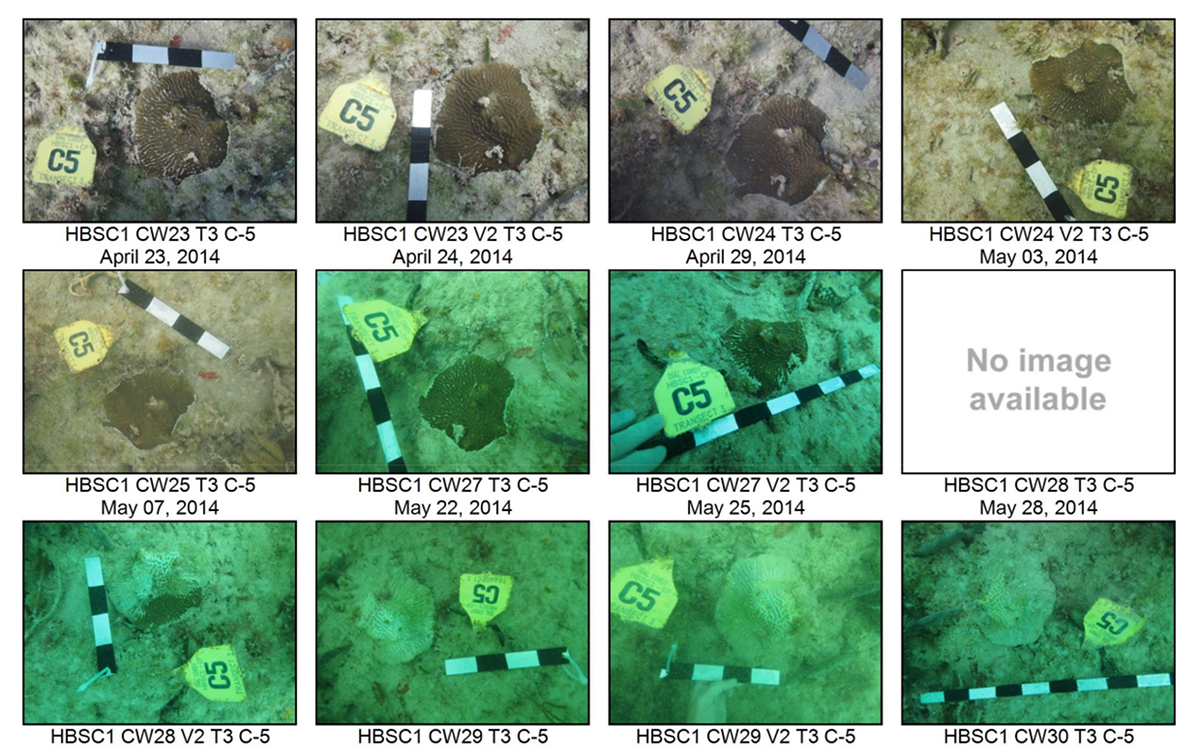
\includegraphics[width=\textwidth]{figures/hbsc1_cp.png}
	\caption{Lightroom photos of tagged corals at site HBSC1-CP \citep{dial2017}. The first signs of the disease appeared between May 25 and May 30. By June 4, the whole colony was completely dead}
\end{figure}
\newpage
\section{Model validation agains tide gauge observations}\label{onset:validation}
\begin{figure}[h!]
    \centering
	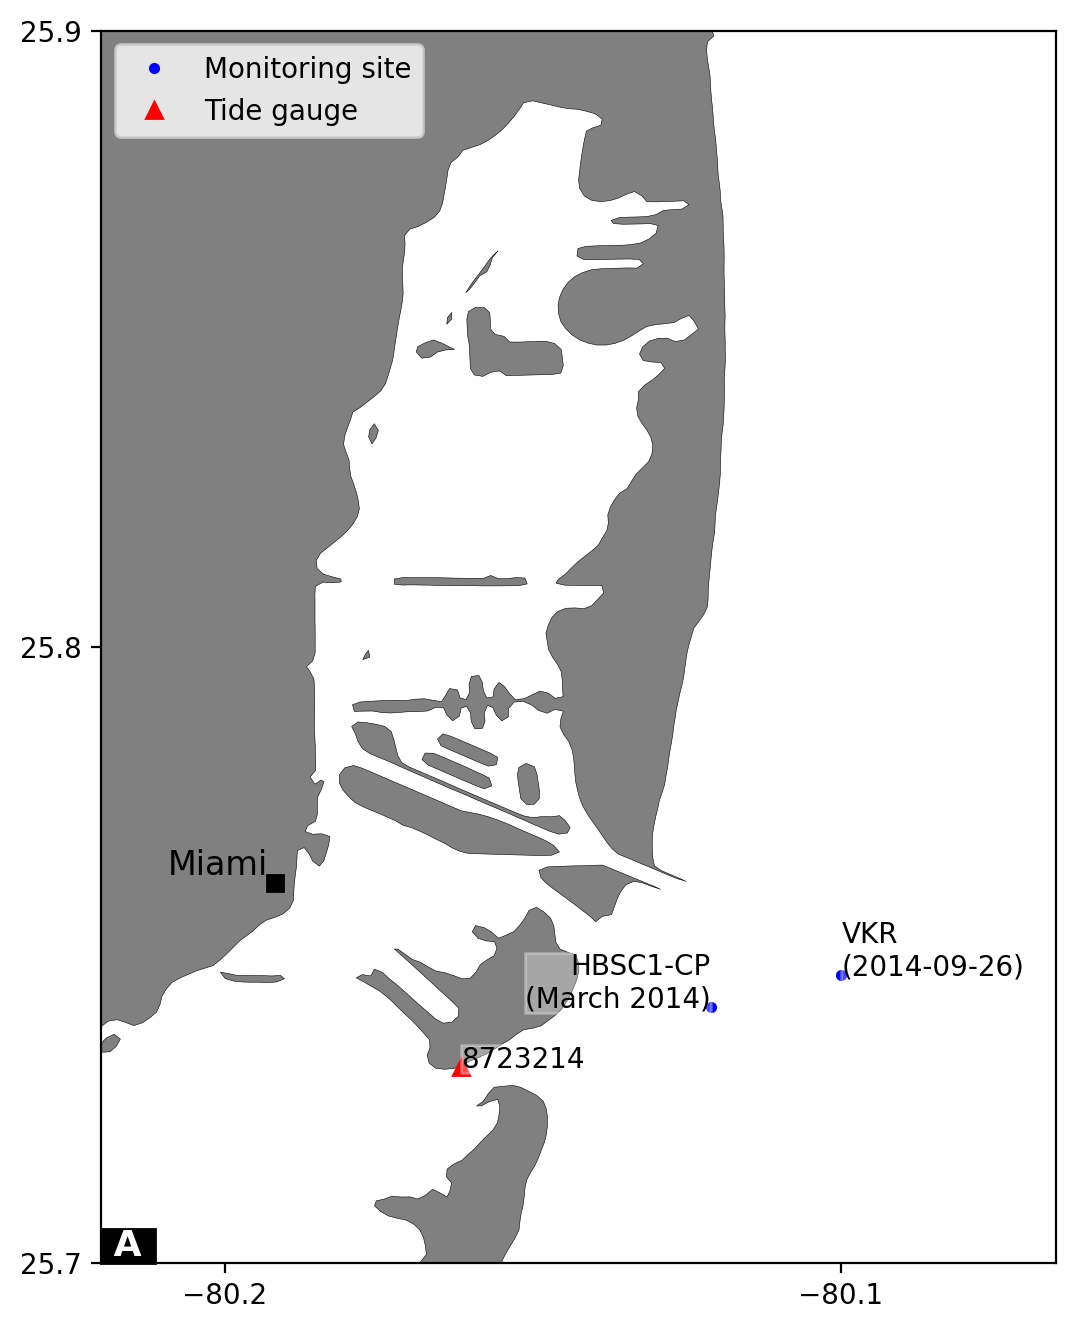
\includegraphics[width=.5\textwidth]{figures/fig_tide_gauge.png}
	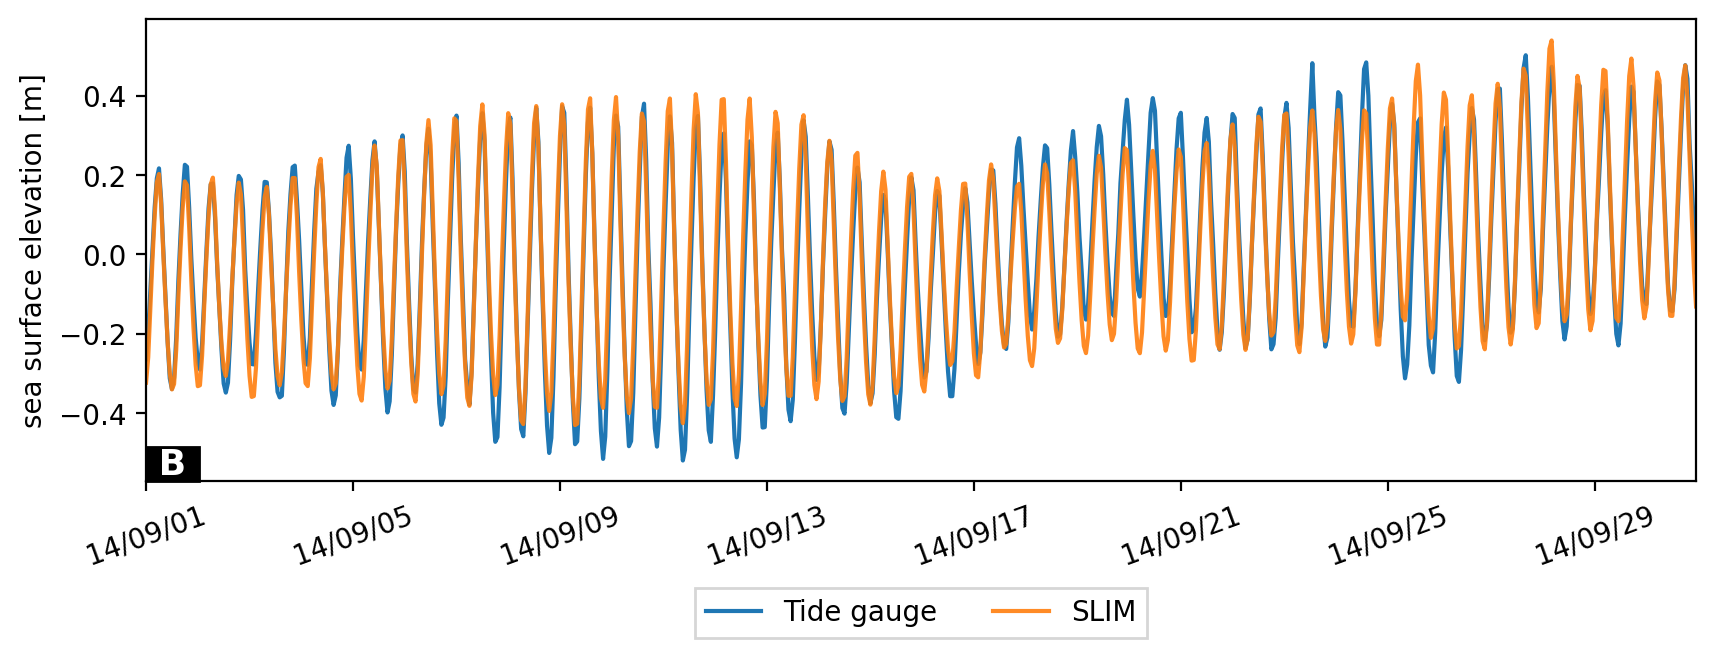
\includegraphics[width=\textwidth]{figures/validation_VK_september.png}
	\caption{\textbf{A}: Location of station 8723214, used to validated the modeled hydrodynamics. \textbf{B}: Comparison of the modeled sea surface elevation against tide gauge observations at station 8723214. The model Root Mean Square Error (RMSE) was 6,7 cm.}
\end{figure}

\end{document}
\endinput
